% !TEX root = ../main.tex
%
\chapter{Search of the \dst dibaryon} \label{sec:4}

\cleanchapterquote{To see a World in a Grain of Sand \\
                   And a Heaven in a Wild Flower \\ 
                   Hold Infinity in the palm of your hand \\
                   And Eternity in an hour}{William Blake}{(Auguries of Innocence)}

In this chapter the details on the data sample and the analysis technique used for the search of the \dst
dibaryon and the related antiparticle, will be presented. 
The \dst has been searched in the \dstdecay decay channel, since this is expected to be the
most relevant channel detectable by the ALICE apparatus \ -- the expected branching ratio is
around 23\% (Tab.~\ref{tab:dst_prop}).

%
%
\section{Analysis strategy} \label{sec:4.1}

This section is dedicated to the detailed description of the strategy adopted in the search of
\dst dibaryon in \pPb collisions at \sctev. 
The data analysis has been performed adopting a \textbf{blind analysis} for the invariant mass distribution
(\minv) of the \ds \textit{candidates}. A \ds \textit{candidate} is a four-vector obtained summing the 
four-momentum of the \ds decay products \ -- therefore $d$, \pip, \pim or the related antiparticles since the
considered decay channel is \dstdecay.
A region of interest in the \minv invariant mass distribution, where the \ds signal is expected to be,
has been defined as follows:
\begin{center}
\textbf{Region of Interest (RoI)}\  $\rightarrow$ \  $(2.280  < $\ \minv$  < 2.480)\ $ \gevcs.
\end{center}
The study of the selection criteria has been conducted without taking into account the RoI. At the end of the selections optimisation the ROI has been \textit{unblinded} and a
background subtraction has been performed to look for the signal.

The idea behind the blind analysis is to optimise the selections and to develop a model
able to describe the background that affects the measurement without introducing any bias. 

The predicted physics properties of the \dst (Sec.~\ref{sec:2}) are summarised in Table~\ref{tab:dst_prop}. 
Considering these values, the chosen RoI ensures that the signal \ -- if this state exists and it is visible with the available statistics
-- \ is basically in that invariant mass interval.
\begingroup
\renewcommand{\arraystretch}{1.5} % Default value: 1
\begin{table}
\centering
\captionsetup{justification=centering}
\begin{tabular}{lr}
\multicolumn{2}{c}{\textbf{Predicted properties}}      \\
\toprule
Mass				                   & 2.380 \ \gevcs   \\
$\Gamma$			        	       & 0.070 \ \gevcs   \\
$d\; \pi^{+} \pi^{-}\ $ B.R.	 & 23(2)\ \%		    \\
\midrule
\end{tabular}
\caption{\dst predicted properties.}
\label{tab:dst_prop}
\end{table}
\endgroup

%
%
\section{Data and Monte Carlo sample} \label{sec:4.2}

The experimental results presented in this thesis are based on the analysis of the data collected with \pPb collisions at \sctev in 2016 by the ALICE experiment at the LHC. 

The data sample  consists of nearly $5.5\times10^{8}$ minimum bias events.
In order to increase the number of collected events, two
different minimum bias triggers have been adopted during this data taking period.
The first trigger, called \code{CENT}, is a minimum bias trigger for the central barrel
detectors. The SDD detector has a high busy time if compared to that of other detectors \ -- around three times
than SSD -- \ which limits the rate of the collected events. 
In order to increase that rate, a second trigger, called \code{FAST}, allows the detection of events coming in the SDD busy time window by excluding the SDD from the data acquisition.
The management of the data flow and these two triggers is performed by the ALICE 
CTP (Sec.~\ref{sec:data_flow}).

In the \textit{off-line} event reconstruction, the whole data set analyzed in this work has been
reconstructed excluding the SDD information from the process, in order to made compatible
the data acquired with the two different triggers.

For this analysis two different Monte Carlo productions have been used.
The first one is a sample of $\sim 5 \times 10^{5}$ \pPb events with injected exotic bound states
and it has been used to study the signal shape and momentum distribution of the \ds, and the reconstruction
efficiency of its decay.
The second one is a sample of $\sim 4.6 \times 10^{7}$ \pPb events and it has been used to study 
the background sources of the measurement.

The Monte Carlo productions are based on the EPOS-LHC generator~\cite{epos_lhc}, which is an event 
generator for minimum bias hadronic interactions, used for both heavy ion interactions and cosmic 
ray air shower simulations.
Since the EPOS-LHC does not include any (anti-)dibaryon, an \textit{ad-hoc} generator was used to
inject \ds and \dsbar, on top of each EPOS-LHC event, in the first Monte Carlo sample mentioned before.
In each generated event ten \dst and ten $\ensuremath{\bar{{d}^{*}}(2380)}$, 
are injected with a flat distribution in transverse momentum \ -- in the $0 \leq \pt \leq 8\;\gevc$ interval
-- \ as well as in the azimuthal angle $\phi$ and in rapidity.
The injected \dst are forced to decay by the generator through the \dstdecay channel. 

The other possible decay of the \dst have not been considered since they are either not relevant or not
detectable \ -- because of the presence of neutral particle in the final state -- \ by ALICE.
Since the considered decay occurs through strong interaction, the decay takes place in the primary
interaction vertex. Therefore the decay products are generated starting from the primary interaction vertex
together with the other collision products.

The transport code used for the generation of the detector response \ -- as described
in Section~\ref{sec:} -- \ is GEANT3~\cite{geant3}. 
The data taking conditions are taken account in the MC by reproducing the configuration of the different 
detectors present during the data taking and hence in the runs used for the data analysis.

\subsection{Monte Carlo validation} \label{sec:4.2.1}

As mentioned above, the EPOS-LHC event generator does not include the \dst dibaryon, therefore it has
been injected on top of the \pPb collisions generated in the Monte Carlo. 
The first step of the search presented in this thesis is the validation of the injection
schema used in the MC through the quality assurance (QA in the following) of the generated MC events.
This validation procedure ensures that the injected dibaryonic states are characterized by the 
physics properties expected for the \dst.

The QA of the Monte Carlo events has been done by checking the shape of the invariant mass distribution
of \dst decay products and using the generated tracks. Only tracks from a \dst and belonging to the
same parent particle have been considered, in order to reduce the background. 

\begin{figure}
    \centering
    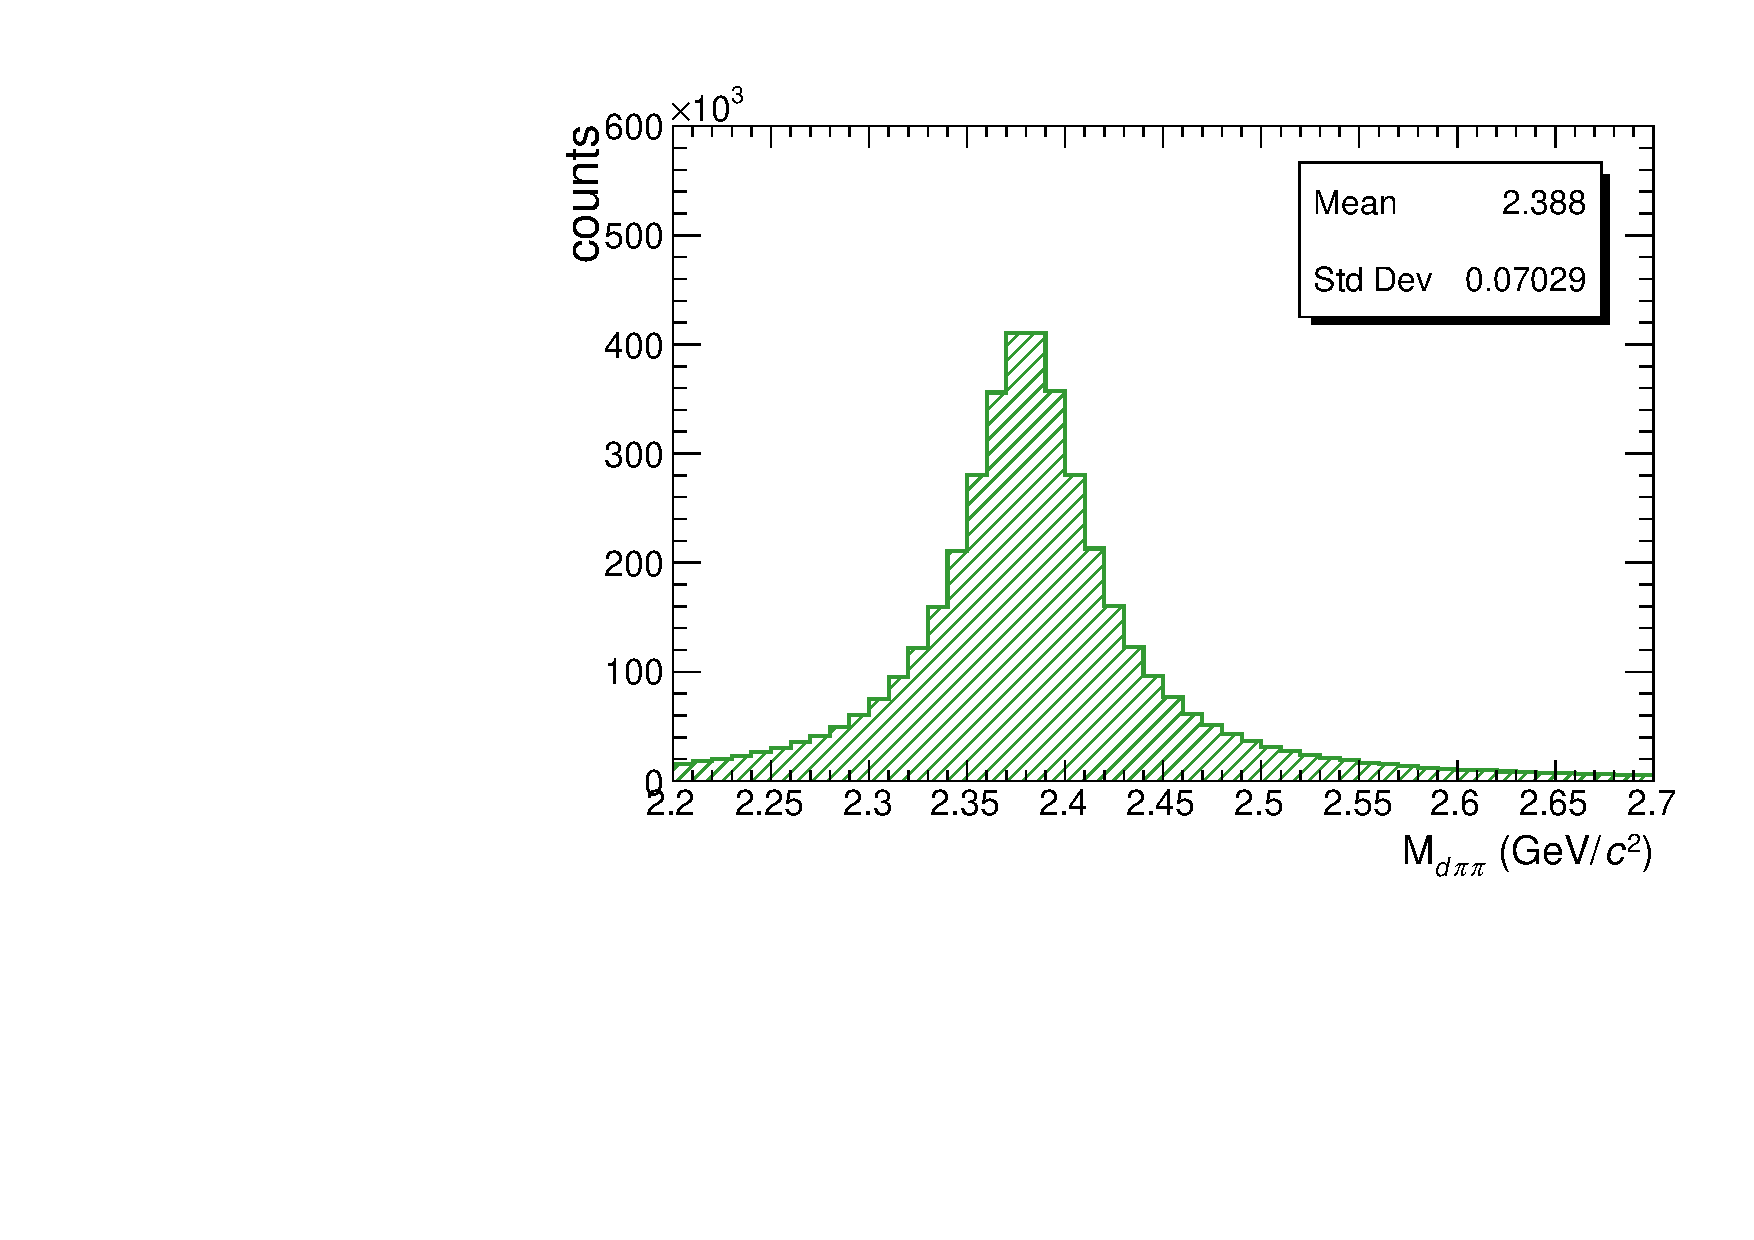
\includegraphics[width=0.8\textwidth]{gfx/valid}
	\caption{Invariant mass distribution of the \dst decay products, obtained by using the generated tracks. The distribution shows the expected shape. The mean and the \textit{rms} of the distribution are compatible with the predicted properties of the \dst.}
	\label{fig:valid}
\end{figure}

The signal observed by the WASA-at-COSY collaboration, as discussed in section~\ref{sec:2.2.2}, has
mass of 2380 \mevcs and a width of $\sim$ 70 \mevcs. Therefore, Figure~\ref{fig:valid} shows that the
injected signal has the mean value of the invariant mass distribution at the correct value expected
for the \dst.

%
%
\section{Event and track selection} \label{sec:4.2}

In this analysis, the events are analysed with the \code{CODEX} framework\footnote{The \code{CODEX} 
framework is part of the \code{AliPhysics} software (Sec.~\ref{sec:anal_frame}) and it is 
specifically developed to provide analysis tools for the ALICE analysis related to nuclei
production.} that allows the selection of events on the basis of the presence of specific particles 
of interest (PoI) in the event and to store them in a compressed format.
Basically, it works as an \textit{off-line} trigger.
Such compressed data can be stored and analysed on local machines, providing an easier and faster
analysis chain.

Using the \code{CODEX} framework, the event and track selection takes part in two different stages.
In the first stage the \code{CODEX} analyses the considered data sample on the
WLCG (Sec.~\ref{sec:offline}) selecting events in which at least one PoI has been reconstructed.
The selected events are filtered by the \code{CODEX} in order to store only

In the second stage the filtered data are analysed on local machines and further track
selections are applied.
In the following sections more details on the event and track selection are provided.

%
\subsection{Event selection: \code{CODEX} filtering}

In the \code{CODEX} filtering the event selection is performed in two steps.
In the first step the events are selected using standard ALICE requirements applied for \pPb collisions.
A selection for the pile-up rejection is applied to exclude events with more than one primary vertex,
while selection based on the resolution and the position of the primary vertex guarantees the goodness of the
reconstructed vertex.
This last selection, basically rejects events for which the position of the vertex reconstructed with full
tracks differs too much from the position of the vertex determined with SPD only.
More details on the two algorithms used to determine the vertex are given in Section~\ref{sec:vertexing}.
The selections applied to the primary vertex in this step of the analysis are summarised in
Table~\ref{tab:cod_sel1}.

\begingroup
\renewcommand{\arraystretch}{1.5} % Default value: 1
\begin{table}[hb]
\centering
\begin{tabular}{lr}
\multicolumn{2}{c}{\textbf{Event selection in \code{CODEX}}}        \\
\toprule
$\mid \textit{z} \mid\ $ primary vertex            & $<$ 10 cm      \\
\textit{z}$_{SPD}$ vertex resolution               & $<$ 0.25 cm    \\
$\mid \textit{z}_{SPD} - \textit{z}_{Track} \mid$  & $<$ 0.5 cm	    \\
\midrule
\end{tabular}
\caption{Event selections, applied in the first step of the \code{CODEX} framework, which ensure a satisfactory reconstruction of the primary vertex.}
\label{tab:cod_sel1}
\end{table}
\endgroup

In the second step a track and particle identification selection with loose cuts is performed.
The concept is to store locally only events with an \textit{(anti-)deuteron candidate}, since without
the (anti-)deuteron the \dst decay cannot be reconstructed.
The expected production rate of (anti-)deuterons in \pPb inelastic collisions is approximately $10^{-4}$,
therefore with this selection it is possible to reduce the number of stored events from at least four
order of magnitude, making the data sample manageable on local machines.

The selection of the \textit{(anti-)deuteron candidate} is based on the $n\sigma\ $ technique, described
in Section~\ref{sec:PID}.
The \textit{(anti-)deuteron candidate} is defined as a track with $n\sigma_{TPC} < 5$ and 
$n\sigma_{TOF} < 10$ with respect to the deuteron mass hypothesis. The requirement on the $n\sigma_{TOF}$
is applied only for tracks with $\pt > 1.5\; \gevc$, since the identification efficiency of the
(anti-)deuteron is higher using the TPC only for tracks with $\pt < 1.5\; \gevc$.

%
\subsection{Track selection} \label{sec:track_sel_crit}

At the end of the event selection, the filtered data are processed on local machines to
define the best set of track selections.
The possibility to analyse on local computing resources the whole data set of interesting events, allows us
to process the data very 
quickly and therefore to study and to easily test further track selections.
In the following the final selections, determined after a fine tuning and a detailed study, are presented.

Since \dstdecay is a strong decay only tracks coming from the primary vertex are 
considered in this analysis. Therefore a selection on the DCA \ -- defined in 
Section~\ref{sec:vertexing} -- \ has been applied. 
In order to use only the geometrical region where the ALICE experiment is able to perform a full
tracking and to provide a PID with high resolution, only tracks in the pseudorapidity 
region $|\eta| < 0.9 $ are selected. This requirement is mainly related to the TPC acceptance,
since it is the main detector used in the present analysis. 
Moreover, to guarantee a track momentum resolution better than 5\% and a TPC \dedx resolution of
6\%, the selected tracks are required to have at least 70 clusters in the TPC and to overcome successfully the ITS and the TPC refit process
\ -- described in Section~\ref{sec:tarcking}.
In addition, the $\chi^{2}$ for TPC clusters is computed in the track fitting procedure and is
required to be less than 4, while the \textit{Golden $\chi^{2}$} \ -- defined as the $\chi^{2}$
between the TPC track constrained to the primary vertex and the global track -- 
\ is required to be less than 36. The selection on the \textit{Golden $\chi^{2}$} value
rejects bad quality primary tracks and also a large fraction of secondary tracks originating from
decay or interaction vertices displaced from the primary vertex.
Finally, a further selection is applied on the \code{kKink} parameter in order to reject
particles coming from beam line interactions.

\begingroup
\renewcommand{\arraystretch}{1.5} % Default value: 1
\begin{table}
\centering
\begin{tabular}{cc}
\multicolumn{2}{c}{\textbf{Track selection criteria}} \\
\toprule
Variable                            &   Selection        \\
\midrule
$\mid \eta \mid$  				    &	$\leq$ 0.9	     \\
TPC clusters	                    &	$>$ 70		     \\
$\chi^{2}$ per TPC clusters		    &	$<$ 4		     \\
Golden $\chi^{2}$                   &   $<$ 36           \\
TPC refit					        &	\code{true}		 \\
ITS refit						    &	\code{true}		 \\
Kink daughters			       		& 	rejected		 \\
DCA$_{xy}$					        &	$<$ $(0.0105+0.0350) / \ensuremath{\pt}^{1.1}$  cm \\
DCA$_{z}$					        &	$<$ 2 cm    	 \\
\midrule
\end{tabular}
\caption{Summary of the track selections applied in the analyses of the 2016 data sample.}
\label{tab:tselection}
\end{table}
\endgroup

The aforementioned track selection criteria are applied to all the studies presented in this
thesis and are summarised in Table~\ref{tab:tselection}.

%
% 
\section{Reconstruction of the \ds} \label{sec:ds_candidate}

After the event and track selection there is nothing left but to determine the (\dsbar)\ds candidates.
This is done by selecting the daughter tracks of the two charged pions decay:
\begin{equation}
    \dstdecay.
\end{equation}
Therefore a (\dsbar)\ds candidate is a triplet of tracks identified as (anti-)deuteron, \pip and
\pim.

The determination of the particle species of the track is performed with a track-by-track
selection on the $n\sigma$ variable as described in Section \ref{sec:PID}. One of the main
challenges in this analysis is to be able to have a good identification of the deuteron in the 
momentum range in which the \ds production is expected to be more abundant. % \ -- $m_{d} >> m_{\pi}\ $ implies that most of the \ds 
% momentum is taken by the deuteron, therefore the deuteron. 
At the same time,
it is essential to have samples of pions and deuterons with high purity.
Therefore the choice of the detectors to be used for the PID is not trivial and needs to
be investigated.

\begin{figure}
    \centering
    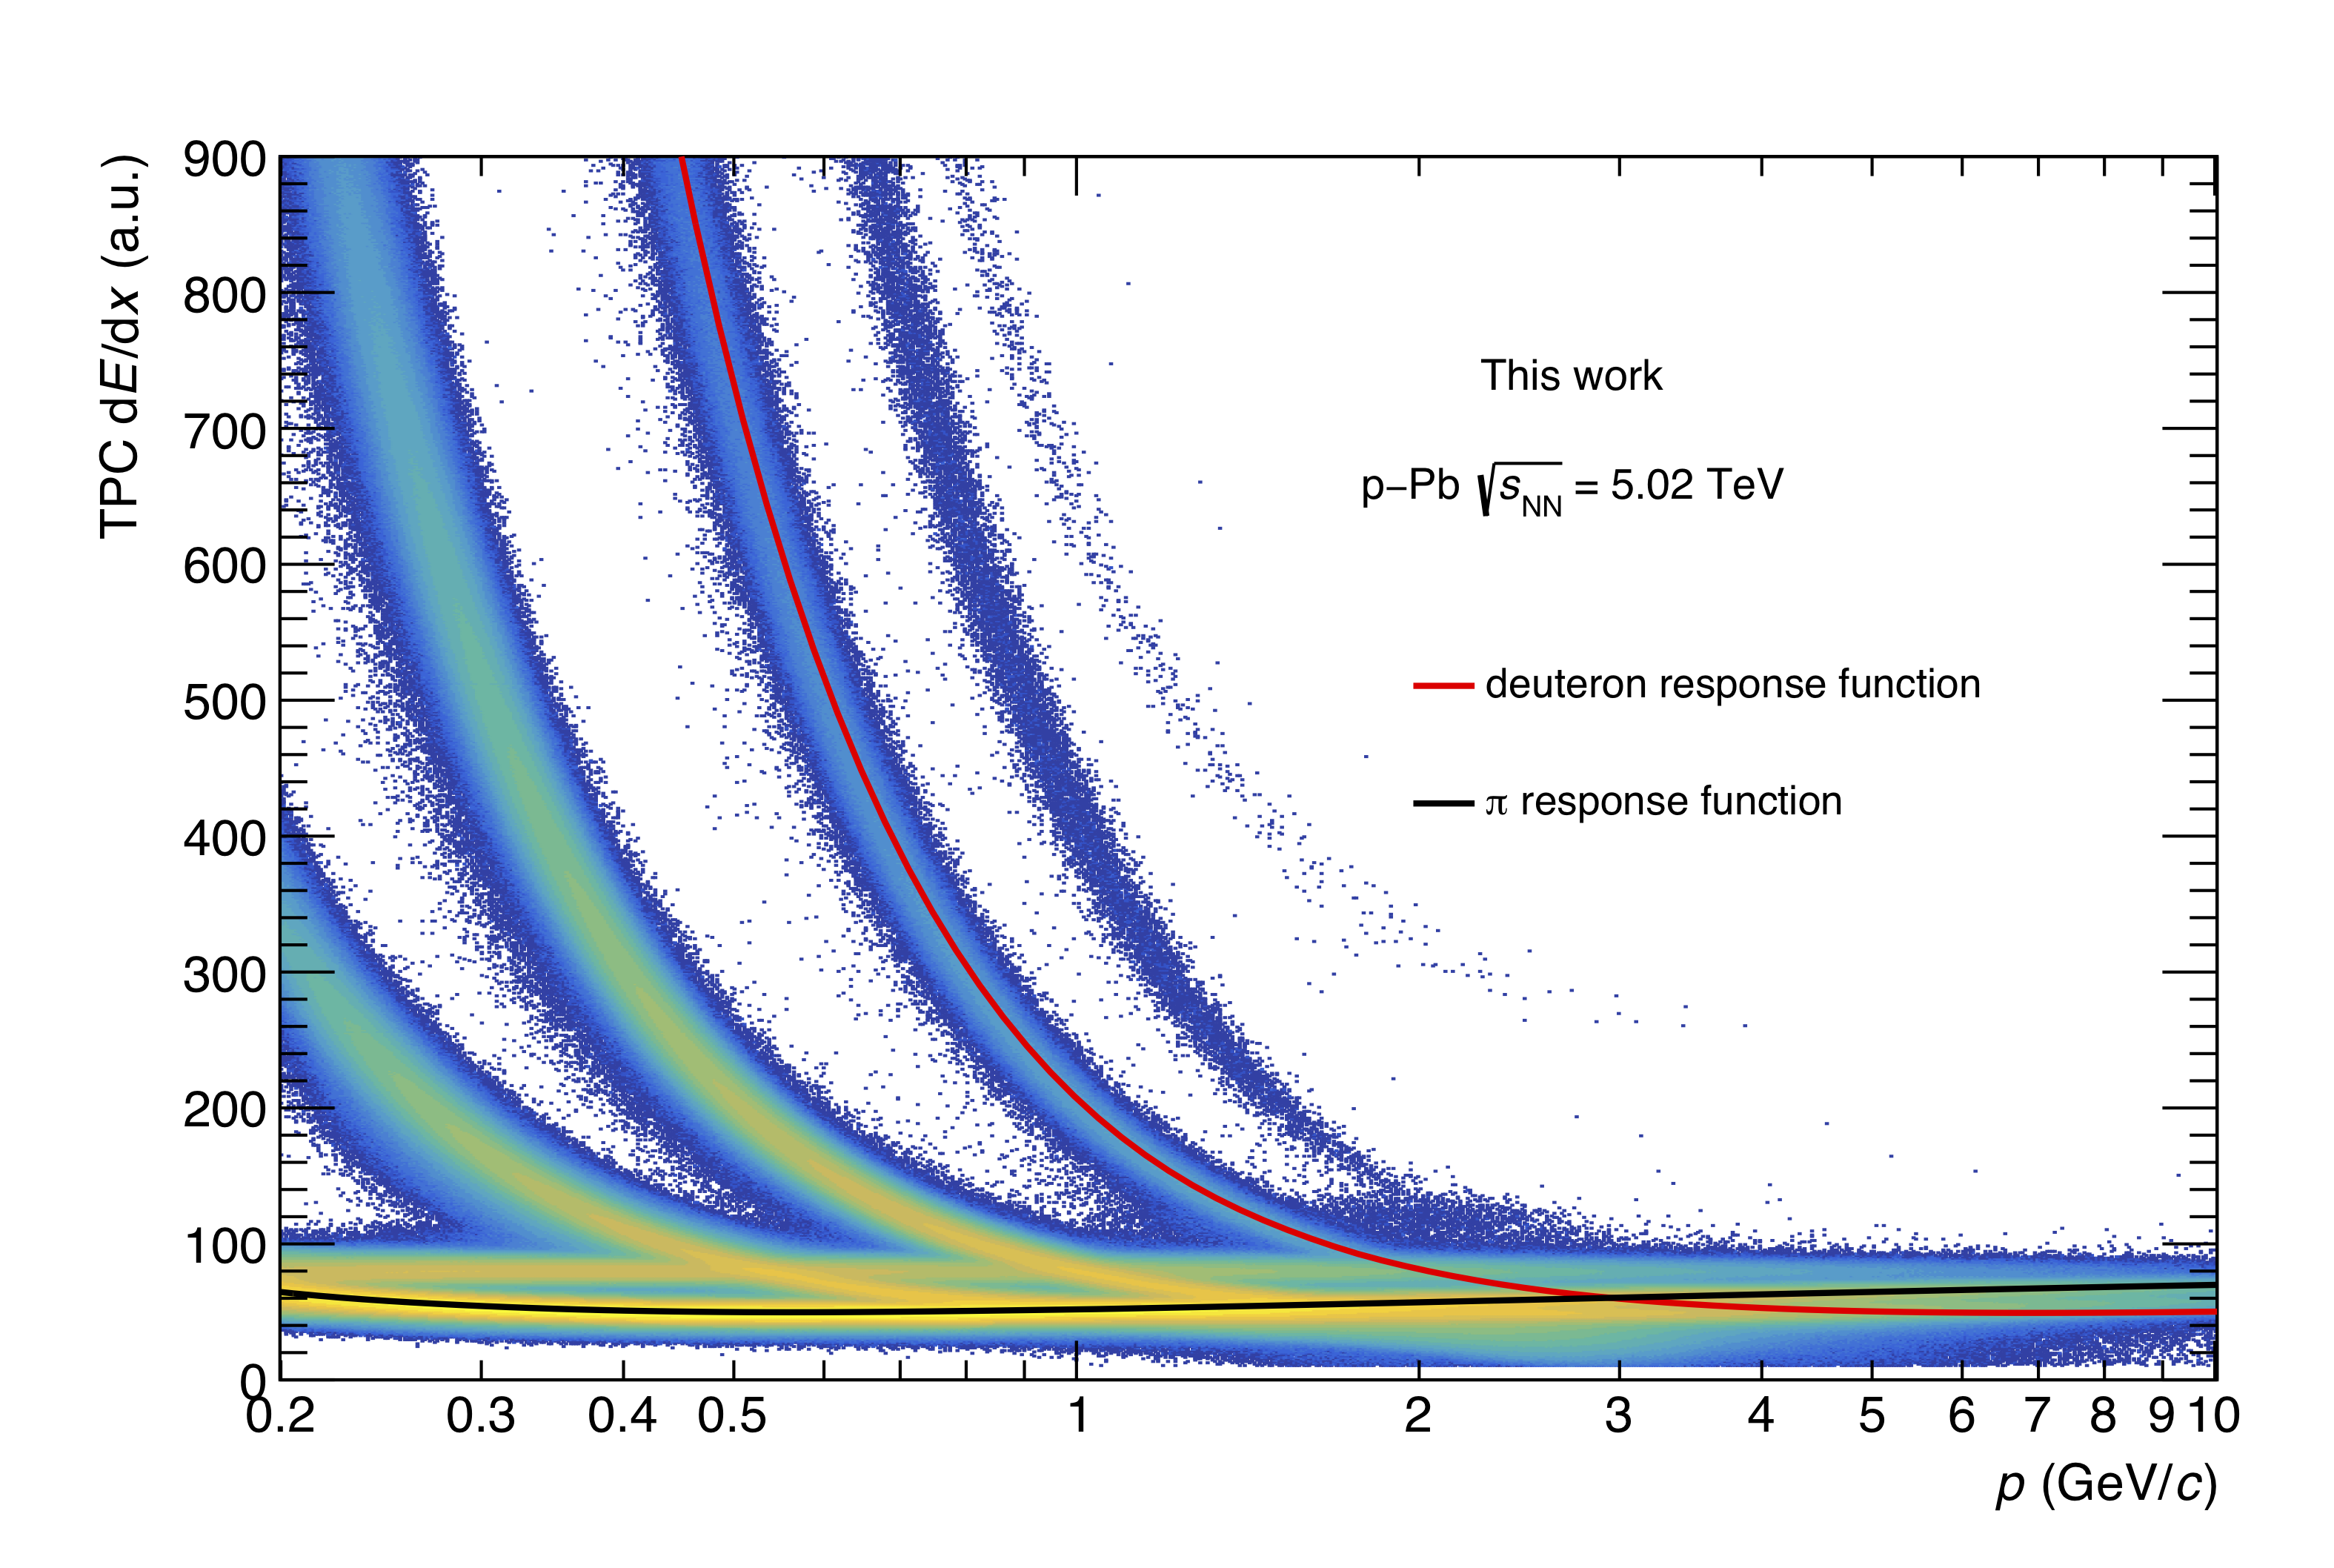
\includegraphics[width=0.8\textwidth]{gfx/pid_tpc}
	\caption{Specific energy loss in the TPC active volume as a function of the particle rigidity in \pPb collisions for the 2016 data sample. The solid lines represent the expected TPC response for pion (black) and deuteron (red).}
	\label{fig:tpc_pid_this}
\end{figure}

A clear identification of the (anti-)deuteron can be performed by using the TPC information only for
tracks up to $p \sim 1.2\; \gevc$, due to the finite resolution on the specific energy loss measured by
the TPC and the contamination from electrons and positrons (Fig.~\ref{fig:tpc_pid_this}).
Using the TOF detector an unambiguous identification of the (anti-)deuteron is feasible for
tracks with momentum up to $p \sim 2\; \gevc$ and a good identification is still doable for tracks up to $p \sim 6\; \gevc$.
Therefore combining TPC and TOF information can improve the performance in terms of PID for particles with enough momentum to 
reach the TOF.

Otherwise the identification of the pion in the TPC is limited by the contamination from kaons and
protons and can be performed for tracks up to $p \sim 1\; \gevc$. Using the TOF for pions
identification can improve the purity of the sample, but at the same time can dramatically reduce
the reconstruction efficiency of the \ds decay, since the pions produced by the \ds are expected to
be at low momentum due to the kinematics of the decay.

In order to determine which PID configuration ensures the best performance in the reconstruction
of the \ds decay, three PID approaches have been studied and are detailed in the following. The choice of the configuration used
for the search of the \ds will be determined on the basis of the best performance reached in the reconstruction of the decay
and taking into account which configuration maximises the signal/background ratio.

\paragraph{PID configurations:}
\begin{itemize}
\item \textbf{TPC:} PID performed only with TPC for both pions and deuterons.
\item \textbf{TPC+TOF:} PID performed with TPC and TOF for both pions and deuterons.
\item \textbf{TPC+TOF$_{deuteron}$:} pions identified with TPC only and deuterons
identified with both TPC and TOF.
\end{itemize}

For each configuration, the same selections are applied on the $n\sigma$ variable as reported in
Table~\ref{tab:pid_config}.

\begingroup
\renewcommand{\arraystretch}{1.5} % Default value: 1
\begin{table}
\centering
\begin{tabular}{ccc}
    \multicolumn{3}{c}{\textbf{PID selections}}  \\%& \multicolumn{2}{c}{\textbf{Selections for TOF}}\\
\toprule
Species & Selection for TPC & Selection for TOF   \\
\hline
$\pi$ & $\mid n \sigma_{TPC}\mid\; \leq 3.$  & $\mid n \sigma_{TOF}\mid\; \leq 3.$ \\

$d$   & $\mid n \sigma_{TPC}\mid\; \leq 3.$  & $\mid n \sigma_{TOF}\mid\; \leq 3.$ \\
\midrule
\end{tabular}
\caption{Selection applied for the identification of candidate $\pi$ and $d$ using the TPC and TOF detectors.}
\label{tab:pid_config}
\end{table}
\endgroup

%
%
\section{Spectrum shape estimation} \label{sec:spectrum}

As reported in Section~\ref{sec:4.2}, in the Monte Carlo productions the \dst was injected with flat
transverse momentum spectrum in the $0 \leq \pt \leq 8\;\gevc$ interval. 
This study is performed in order to have a more realistic spectrum both for the \ds and for the decay 
products.

Assuming the same \pt spectrum of the deuteron for the \ds, it is possible to obtain the \ds 
transverse momentum spectrum with a rejection sampling. The deuteron spectrum in \pPb collisions is
described by the Blast Wave (BW) distribution, which is based on the phenomenological model for
hadronic matter production in heavy ion collisions, published in Ref.~\cite{blastwave}.
The distribution is written as:
\begin{equation}
    \frac{1}{\pt} \frac{d\,N}{d\,\pt} \propto \int_{0}^{R} r\,dr\,m_{\mathrm{T}} I_{0}
    \left( \frac{\pt \sinh\rho}{T_{kin}} \right) K_{1} \left( \frac{m_{\mathrm{T}} \cosh\rho}
    {T_{kin}} \right),
\end{equation}
where the parameter $\rho$ contains the dependence on the velocity profile, since it is expressed
as:
\begin{equation}
    \rho = \tanh^{-1} \left[ \left( \frac{r}{R} \right)^{n} \beta_{s} \right]
\end{equation}
In the previous equations $m_{\mathrm{T}} = \sqrt{\pt^{2} + m^{2}}$ is the transverse mass,
$I_{0}$ and $K_{1}$ the modified Bessel functions, $r$ is the radial distance on the transverse plane,
$T_{kin}$ is the kinetic freeze-out temperature, $\beta_{s}$  the surface velocity of the expanding 
medium and $n$ is the exponent of the velocity profile.
The parameter values, used in this analysis and summarised in Table~\ref{tab:bw_param}
were obtained by fitting the measured deuterons spectrum with the BW distribution in previous
analysis. % citare da dove vengono questi parametri
\begingroup
\renewcommand{\arraystretch}{1.5} % Default value: 1
\begin{table} [htb]
\centering
\begin{tabular}{lc}
\multicolumn{2}{c}{\textbf{Blast wave parameters}} \\
\toprule
Parameter       &   Value            \\
\midrule
$m$			    &	1.8756 \gevcs    \\
$n$             &   1.97208          \\
$T_{kin}$       &   0.128583         \\
$\beta_{s}$     &   0.710369         \\
\midrule
\end{tabular}
\caption{Values of the parameters of the Blast Wave distribution used, in this analysis, as a basis fo the rejection method implemented to obtain a realistic spectrum for the \ds in the Monte Carlo.}
\label{tab:bw_param}
\end{table}
\endgroup

\begin{figure} [htb]
    \centering
    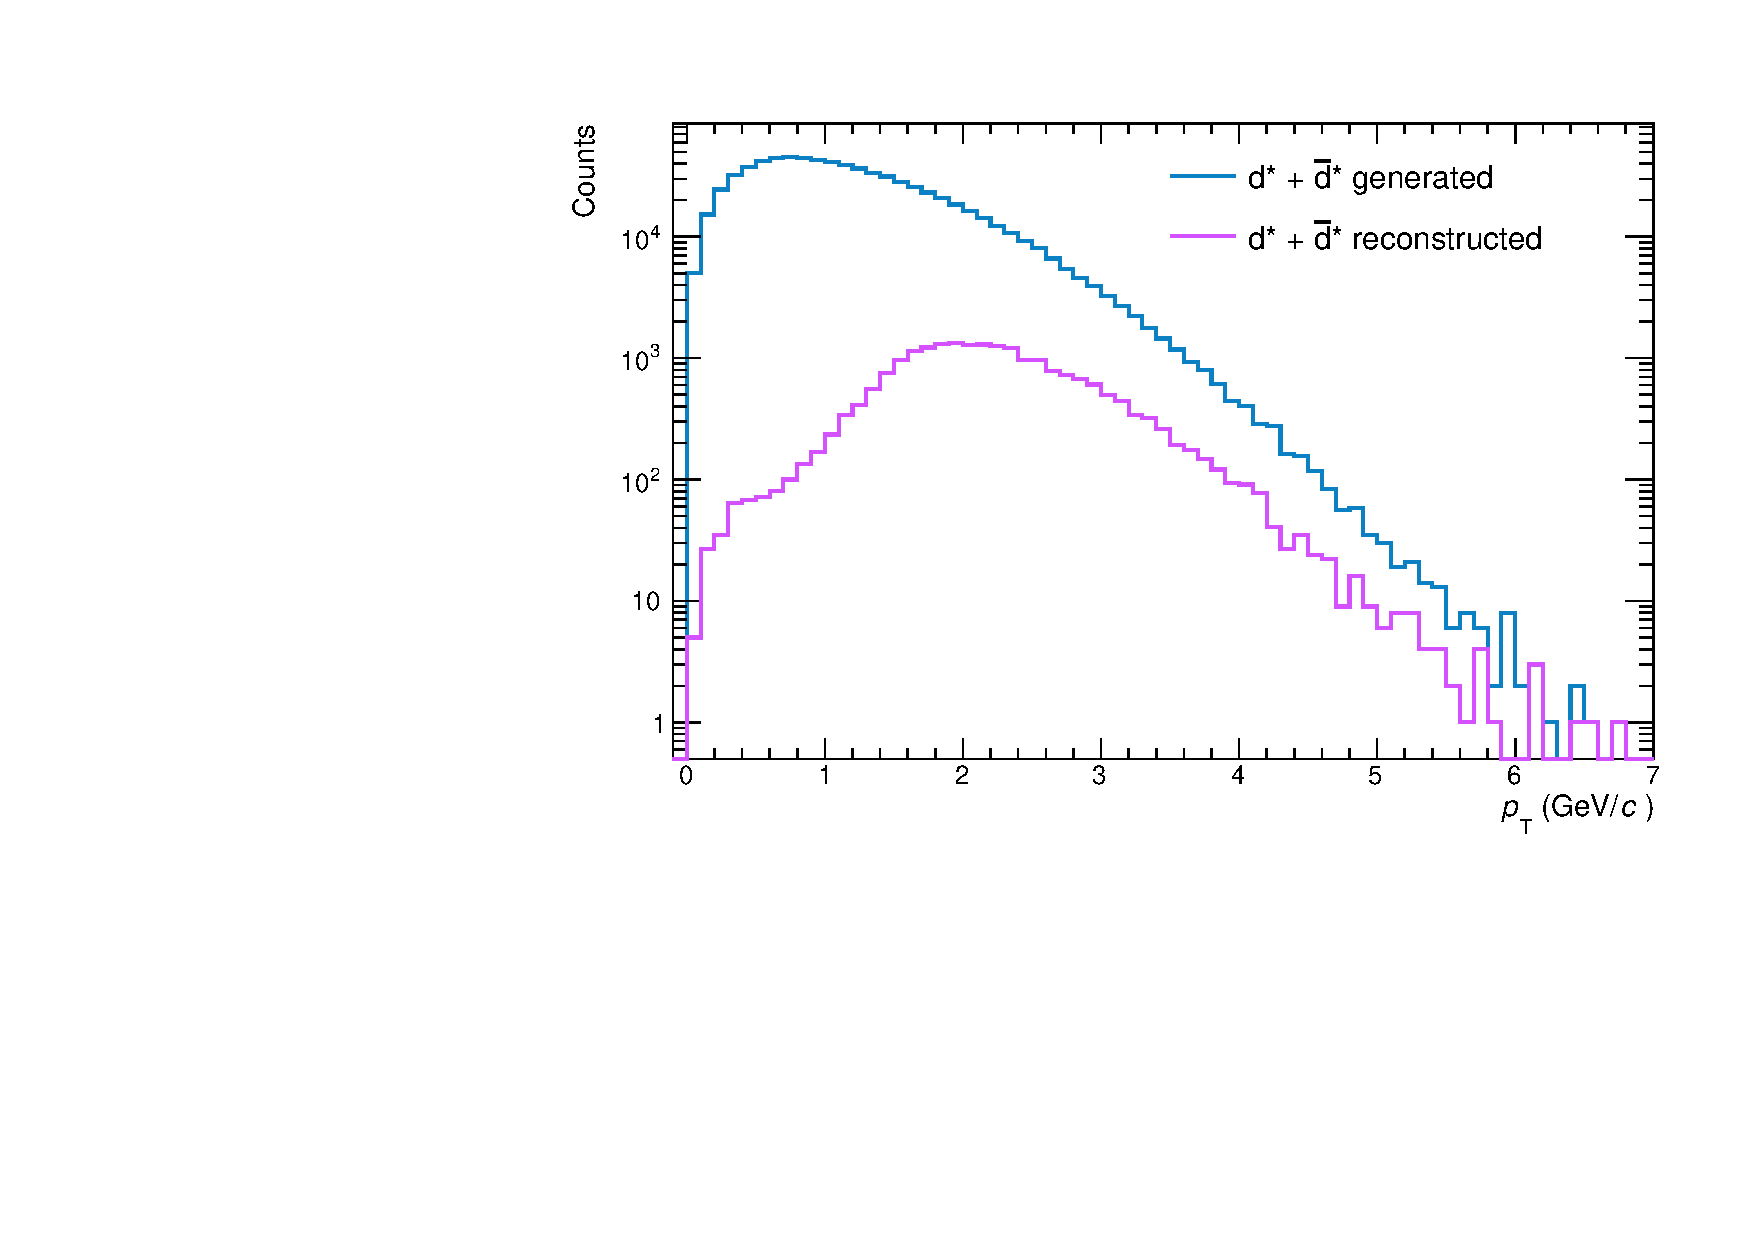
\includegraphics[width=0.7\textwidth]{gfx/genrecBW}
	\caption{Spectrum for both generated (blue line) and reconstructed (magenta line) \ds obtained with Blast Wave rejection sampling.}
	\label{fig:bw_spectrum}
\end{figure}

The rejection sampling has been applied to the \ds generated in the Monte Carlo, obtaining a 
plausible \pt spectrum for the \ds and its decay products. In Figure~\ref{fig:bw_spectrum} the
resulting \pt spectrum for the \ds is shown both before (blue line) and after (magenta line) the
reconstruction process. 
In Figure~\ref{fig:BW_spec_prod} the expected momentum spectra of the pions 
(Panel~\ref{fig:pi_spectrum}) and the deuterons (Panel~\ref{fig:deu_spectrum}) originating from
the \ds decay are reported.

\begin{figure}[htb]
\begin{subfigure}{.5\textwidth}
  \centering
  \captionsetup{justification=centering}
  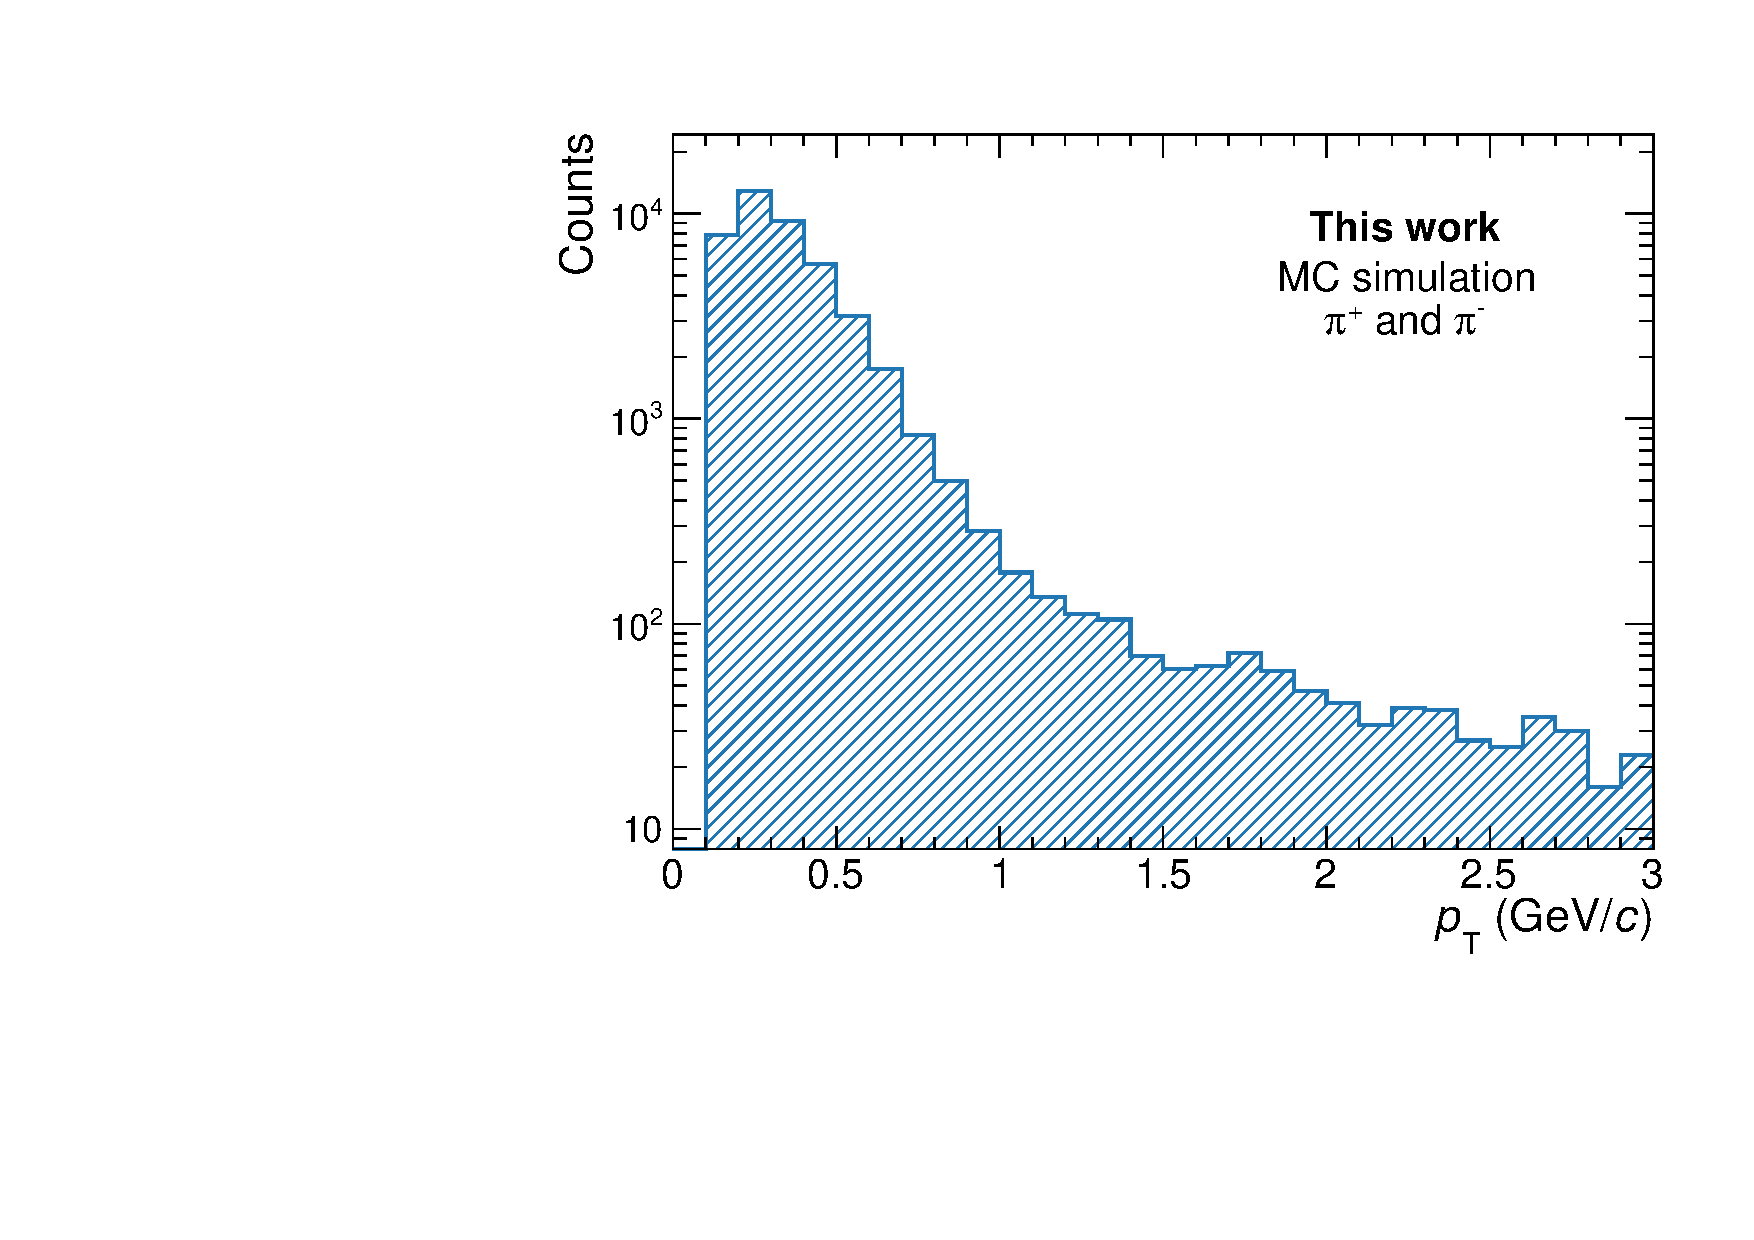
\includegraphics[width=\linewidth]{gfx/pi_spectrum}
  \caption{}
  \label{fig:pi_spectrum}
\end{subfigure}%
\begin{subfigure}{.5\textwidth}
  \centering
  \captionsetup{justification=centering}
  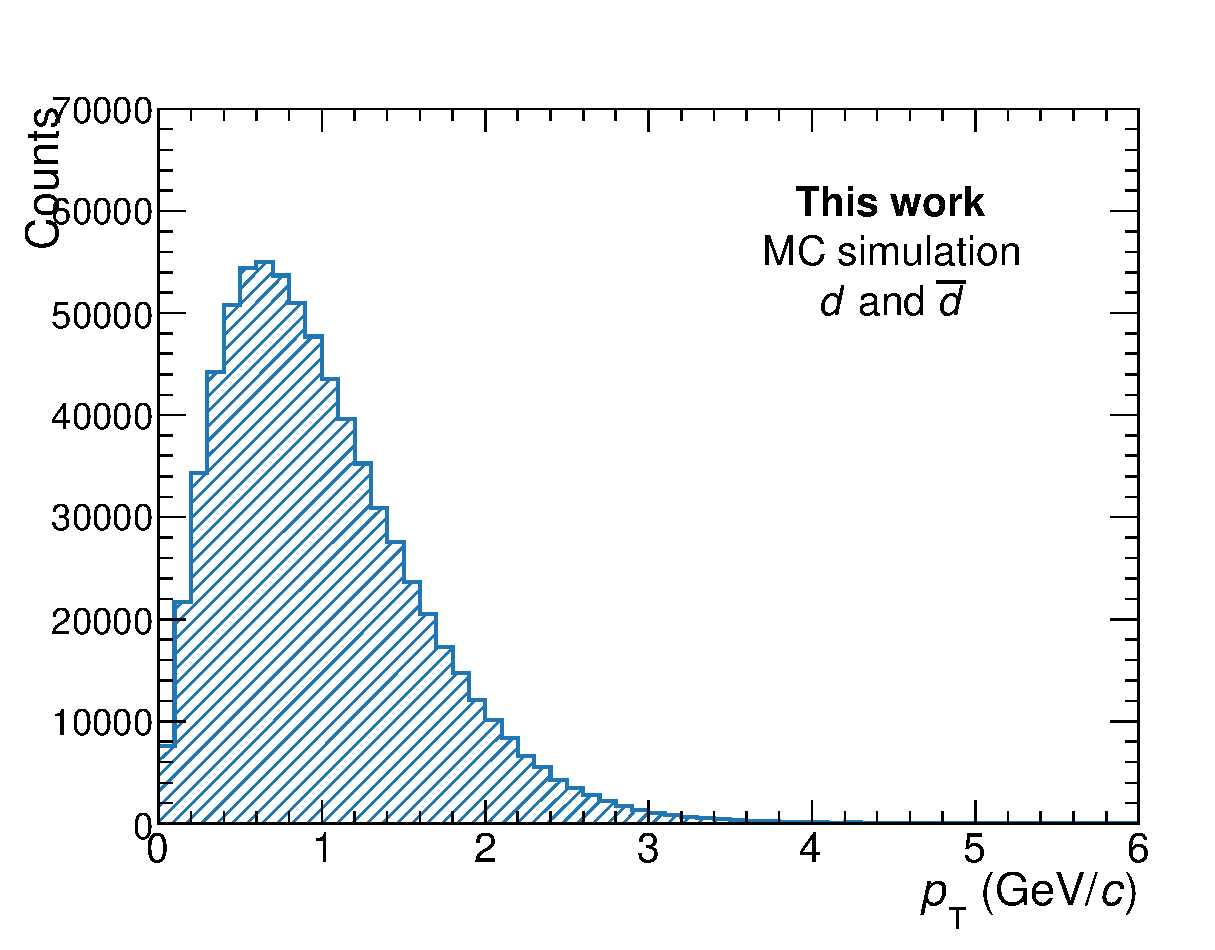
\includegraphics[width=\linewidth]{gfx/deu_spectrum}
  \caption{}
  \label{fig:deu_spectrum}
\end{subfigure}
\caption{Expected transverse momentum spectrum for the \ds decay products derived with the rejection sampling: pions in panel (a) and deuterons in panel (b).}
\label{fig:BW_spec_prod}
\end{figure}

%
%
\section{Reconstruction efficiency of the \ds decay}~\label{sec:eff}

One of the fundamental steps of the analysis presented in this thesis is to evaluate if the
\dstdecay is detectable by the ALICE apparatus, considering the reconstruction efficiency and the acceptance
of the ALICE detectors. 

Furthermore, if the decay is visible, the measured yields are biased by inefficiencies in the
ALICE detectors.
For instance, the active area of the experiment is not hermetic by design or, sometimes, parts of
the detectors might be switched off during some data taking periods due to technical problems,
reducing the efficiency.
The acceptance, instead, is only related to the geometric coverage of the detectors.

It is possible to correct for the finite efficiency and acceptance using a MC simulation where the
full geometry and the real data taking conditions are reproduced. The MC production used for this
analysis has been described in Section~\ref{sec:4.2}. 
The number of particles crossing the detectors and their kinematic observables are known when using
the MC simulation and the efficiency$\times$acceptance can be computed as:
\begin{equation}
    Efficiency \times Acceptance\ (\pt) = \frac{\mathrm{N}_{\textit{rec}}(\pt)}
    {\mathrm{N}_{\textit{gen}}(\pt)},
\end{equation}
where $\mathrm{N}_{\textit{gen}}$ is the number (\dsbar)\ds generated in the azimuthal region
$0 \leq \phi < 2\pi$ for $|y| < 0.5$, while $\mathrm{N}_{\textit{rec}}$ is the number of 
(\dsbar)\ds for which the decay products satisfy the selection criteria described in 
Section~\ref{sec:track_sel_crit}.

Since anti-deuterons can be absorbed by detector material, the efficiency for \dsbar is
expected to be lower than \ds.
Therefore the $Efficiency \times Acceptance$ is evaluated for \ds and \dsbar separately as a
function of the transverse momentum for the three PID configurations. 
The results are shown in Figure~\ref{fig:effAM}.

The TPC only configuration has the highest efficiency,
but in the light of the considerations of Section~\ref{sec:ds_candidate} has also a high 
contamination of the deuteron sample at high momentum.
The TPC-TOF configuration has a very low efficiency, due to the high pions suppression 
resulted from the use of TOF for their identification. 
Instead the TPC+TOF$_{deuteron}$ configuration guarantees a good efficiency and should also ensures
a better deuteron sample purity than the TPC configuration.

The choice of the PID configuration, thus, will be done after the study of the significance of the measurement ensured by the two different configurations.

\begin{figure}
    \centering
    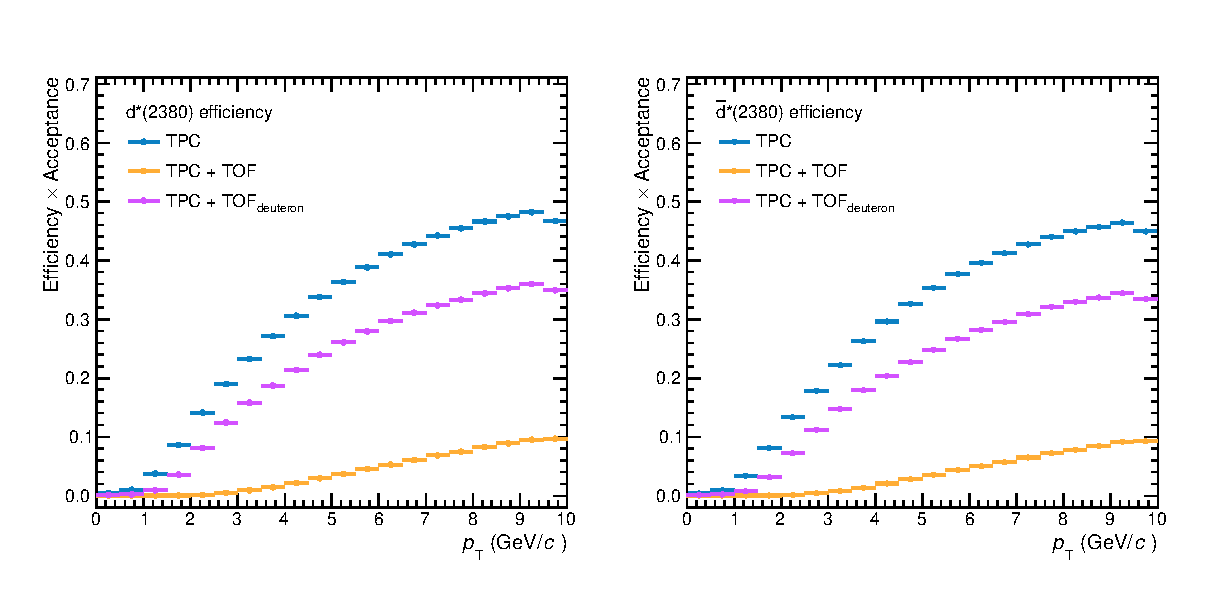
\includegraphics[width=\textwidth]{gfx/eff3globalSLIM}
	\caption{Reconstruction efficiency of the \ds (left panel) and \dsbar (right panel) decay as a function of the transverse momentum for the three considered PID configurations.}
	\label{fig:effAM}
\end{figure}

A more accurate evaluation of the discrepancy between \ds and \dsbar efficiency has been done
by computing the \ds/\dsbar efficiency ratios for all the PID configurations.
In Figure~\ref{fig:eff_ratioAM} the ratio computed for TPC+TOF$_{deuteron}$ is reported.

\begin{figure} [!h]
    \centering
    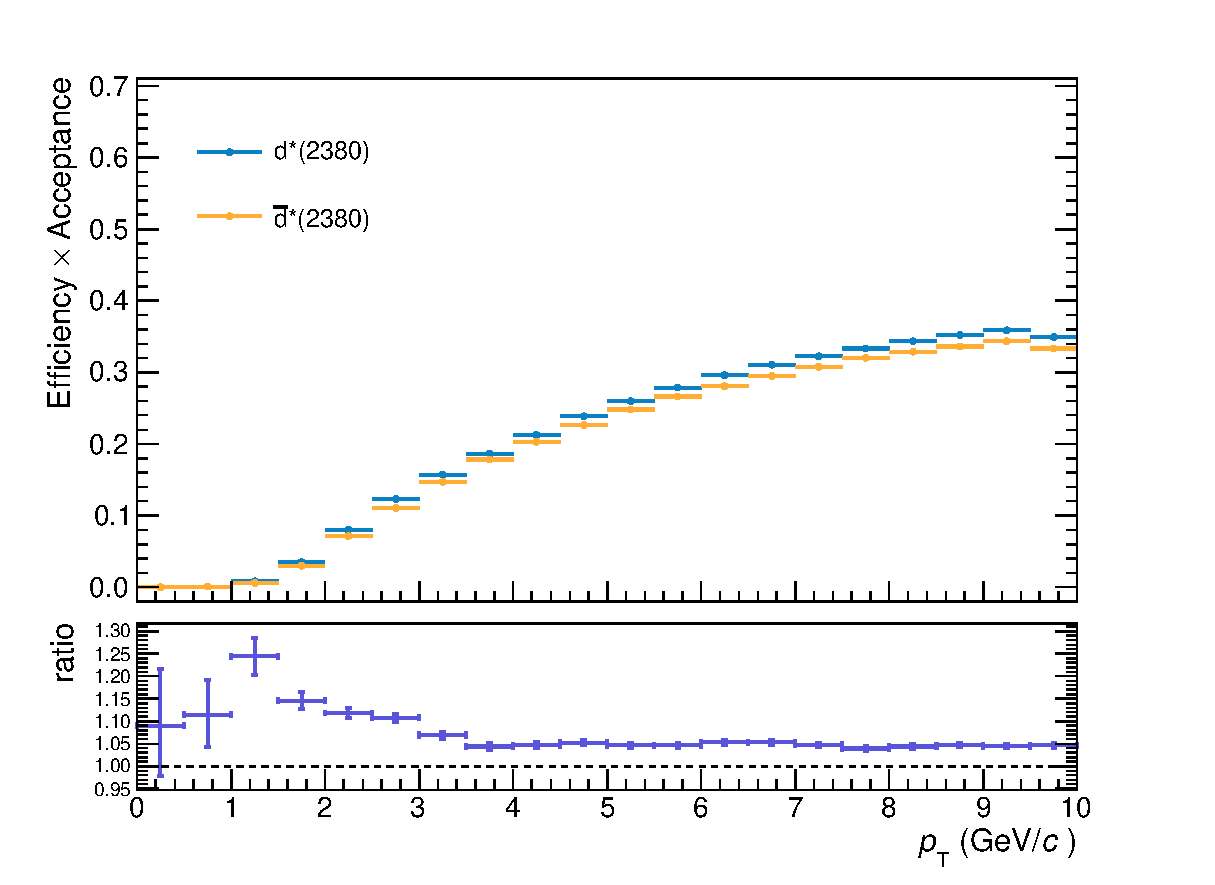
\includegraphics[width=0.8\textwidth]{gfx/eff_ratioAM1SLIM}
	\caption{The efficiency $\times$ acceptance for both \ds and \dsbar is compared for the TPC+TOF$_{deuteron}$ configuration. The \ds/\dsbar efficiency ratio is also reported and shows a behaviour compatible with what expected from the anti-deuteron cross section with material.}
	\label{fig:eff_ratioAM}
\end{figure}

The relative difference between \ds and \dsbar efficiency is higher than $10$ \% and reaches 
a maximum value of $25$ \% for $\pt < 3\;\gevc$, instead at higher \pt is $\sim 6\ $\%. 
These values are compatible with what is expected from the anti-deuteron cross section with material,
that decreases at higher \pt.

The determination of which PID configuration shall be chosen
must be made considering the momentum region in which the \ds is expected to be produced more 
abundantly.
In the light of the study of the expected \ds momentum spectrum (Sec.~\ref{sec:spectrum}), the 
crucial region for the efficiency is the $0 - 2\;\gevc$ \pt interval.
Therefore the TPC/TPC+TOF$_{deuteron}$ efficiency ratio has been computed and compared with the expected
\ds transverse momentum spectrum.
The Figure~\ref{fig:eff_spec} shows the comparison between this two configurations and the expected \pt
spectrum of the \ds.

\begin{figure}
    \centering
    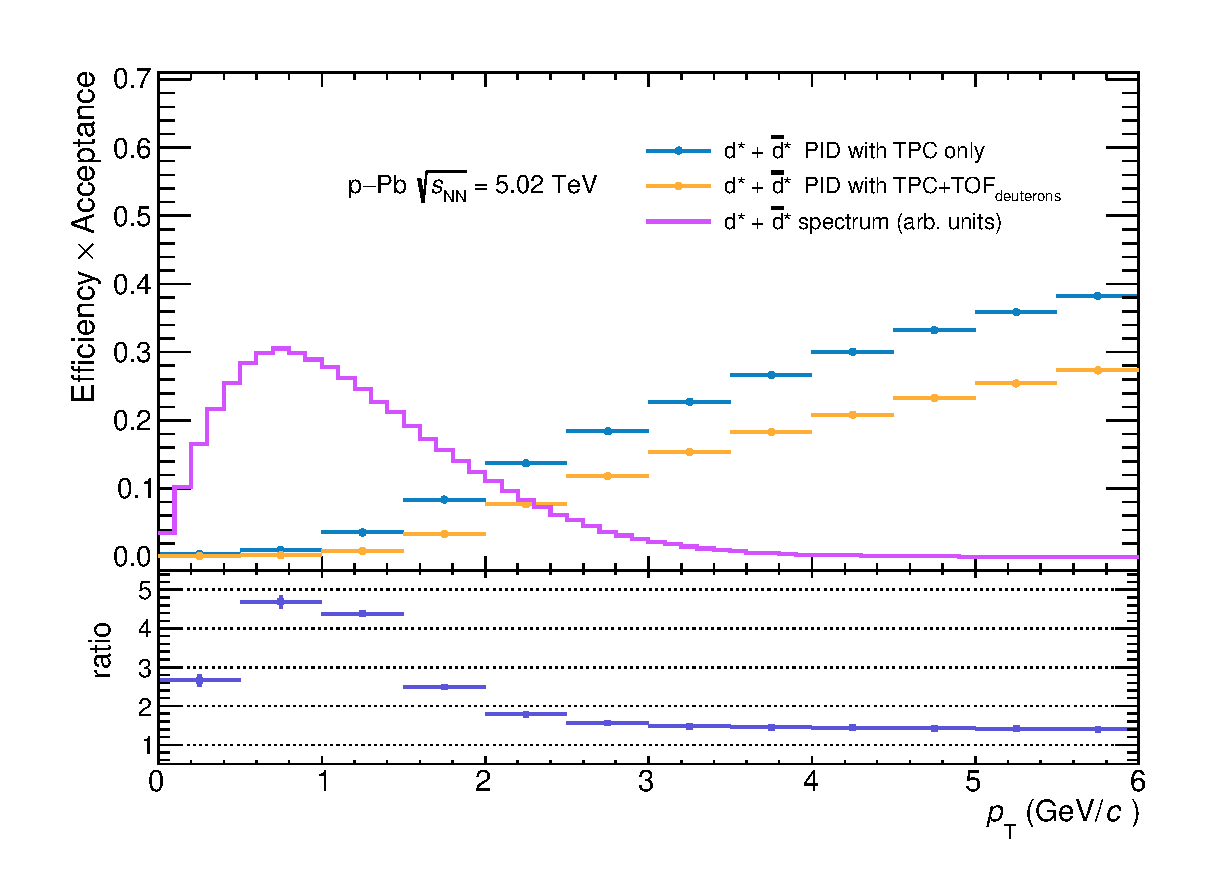
\includegraphics[width=0.8\textwidth]{gfx/effspecSLIM}
	\caption{The expected \pt distribution for the \ds derived in Section ~\ref{sec:spectrum} is superimposed to the efficiency computed for TPC and TPC+TOF$_{deuteron}$ PID configurations. The ratio between the efficiencies of the two configurations is also reported.}
	\label{fig:eff_spec}
\end{figure}

Both the TPC and TPC+TOF$_{deuteron}$ configurations have low efficiencies ($< 0.02$) in the $0 - 1\;\gevc$
interval. While in the $1 - 2\;\gevc$ interval the TPC configuration efficiency reaches the value of 0.10.
In the whole $0 - 2\;\gevc$ interval the TPC efficiency is 3-5 times higher than the obtained with TPC+TOF$_{deuteron}$.

Nevertheless, the choice of which PID configuration should be used is still not trivial. 
In order to observe the \ds signal, it is crucial to have a good signal/background ratio that depends
both on the efficiency and on the purity of considered sample.
The usage of the TOF for the identification of the deuteron ensures a reduced contamination \ -- from 
other particle species -- \ of the deuteron sample. 
Therefore the TPC+TOF$_{deuteron}$ configuration should have better performance in terms of the 
signal/background ratio, respect to the TPC configuration.

%
%
\section{Study of the background of the measurement} \label{sec:background}

In order to perform the background subtraction described in Section~\ref{sec:4.1} it is necessary to have
a model that satisfactorily reproduces the background of the measurement. 
Therefore two different background models have been developed and tested. 
In this section the models and their performance in describing the background are discussed.

In this work the main difficulty is to manage to describe and reproduce the background due to pions.
Indeed, in \pPb collisions many particle species are produced~\cite{pkp_prod, neutralp, k0s_prod} 
and most of them have a decay channel that include a charged pion.
In particular neutral mesons, e.g. $\eta,\,\omega,\,K_{s}^{0}$ mesons, have a 
\pip + \pim decay channel. Other pions, as well as deuterons, can be produced directly
in the hadronization phase of the collision.
All of these pions and deuterons contribute to the background of the measurement of the
\dstdecay decay. In fact one can make a \textit{\ds candidate} (Sec.~\ref{sec:ds_candidate})
matching particles not originating from a real \ds decay.

The two models are both based on the event mixing technique.
Event mixing, basically, is a method used to reproduce uncorrelated background combining particles from
different events, this ensures that there can not be correlation between the considered particles.
This technique can be very effective, but it is necessary to be careful in mixing particles from 
similar events.
So it is very important to mix particles from events with comparable vertices and particle multiplicity 
and to study the performance of this method with different classifications of similar events.

Event mixing can be very expensive in terms of memory usage, because it is necessary to store
lots of events that will later be combined with others.
The tool used to store events is part of the \code{CODEX} framework and has been specifically 
developed for providing an efficient memory usage.
Different event classifications were studied for both models, in order to find the setup that 
guarantees the best background description.

%
\subsection{Partial Event Mixing model} \label{sec:pem}

In order to reproduce both correlated and uncorrelated backgrounds a model has been developed combining pion 
pairs from one event with deuterons from another. In the following this model will be referred as the 
partial event mixing model (PEM).
In principle this model ensures to break the correlation between \textit{\ds candidates} because at least one
out of three particles is taken from a different event.
At the same time, it should correctly describe the correlations between pions because they are taken 
from the same event.
Events are classified by the position of the vertex along the $z$ axis ($z_{vertex}$) only.
Classification in terms of particle multiplicity of the event was tested, but has not been used because
does not improve the background description.
Different $z_{vertex}$ classifications have been studied and the final choice is a $10\ $ class of $2\;$ cm
classification in the $-10 < z_{vertex} < 10$ cm interval.
For each event, every pion pairs is combined with 5 different deuterons from 5 different events
with $z_{vertex}$ in the same class.

The model is compared with the \minv distribution \ -- outside the region of interest -- \ in
0.5 \gevc intervals of the transverse momentum of the \textit{\ds candidates}. 
Since the \ds production is expected to be negligible for $\pt > 5$ \gevc , the comparison between the
model and the \minv has been performed only for \textit{\ds candidates} with transverse momentum under
this value.

\begin{figure} [htb]
    \centering
    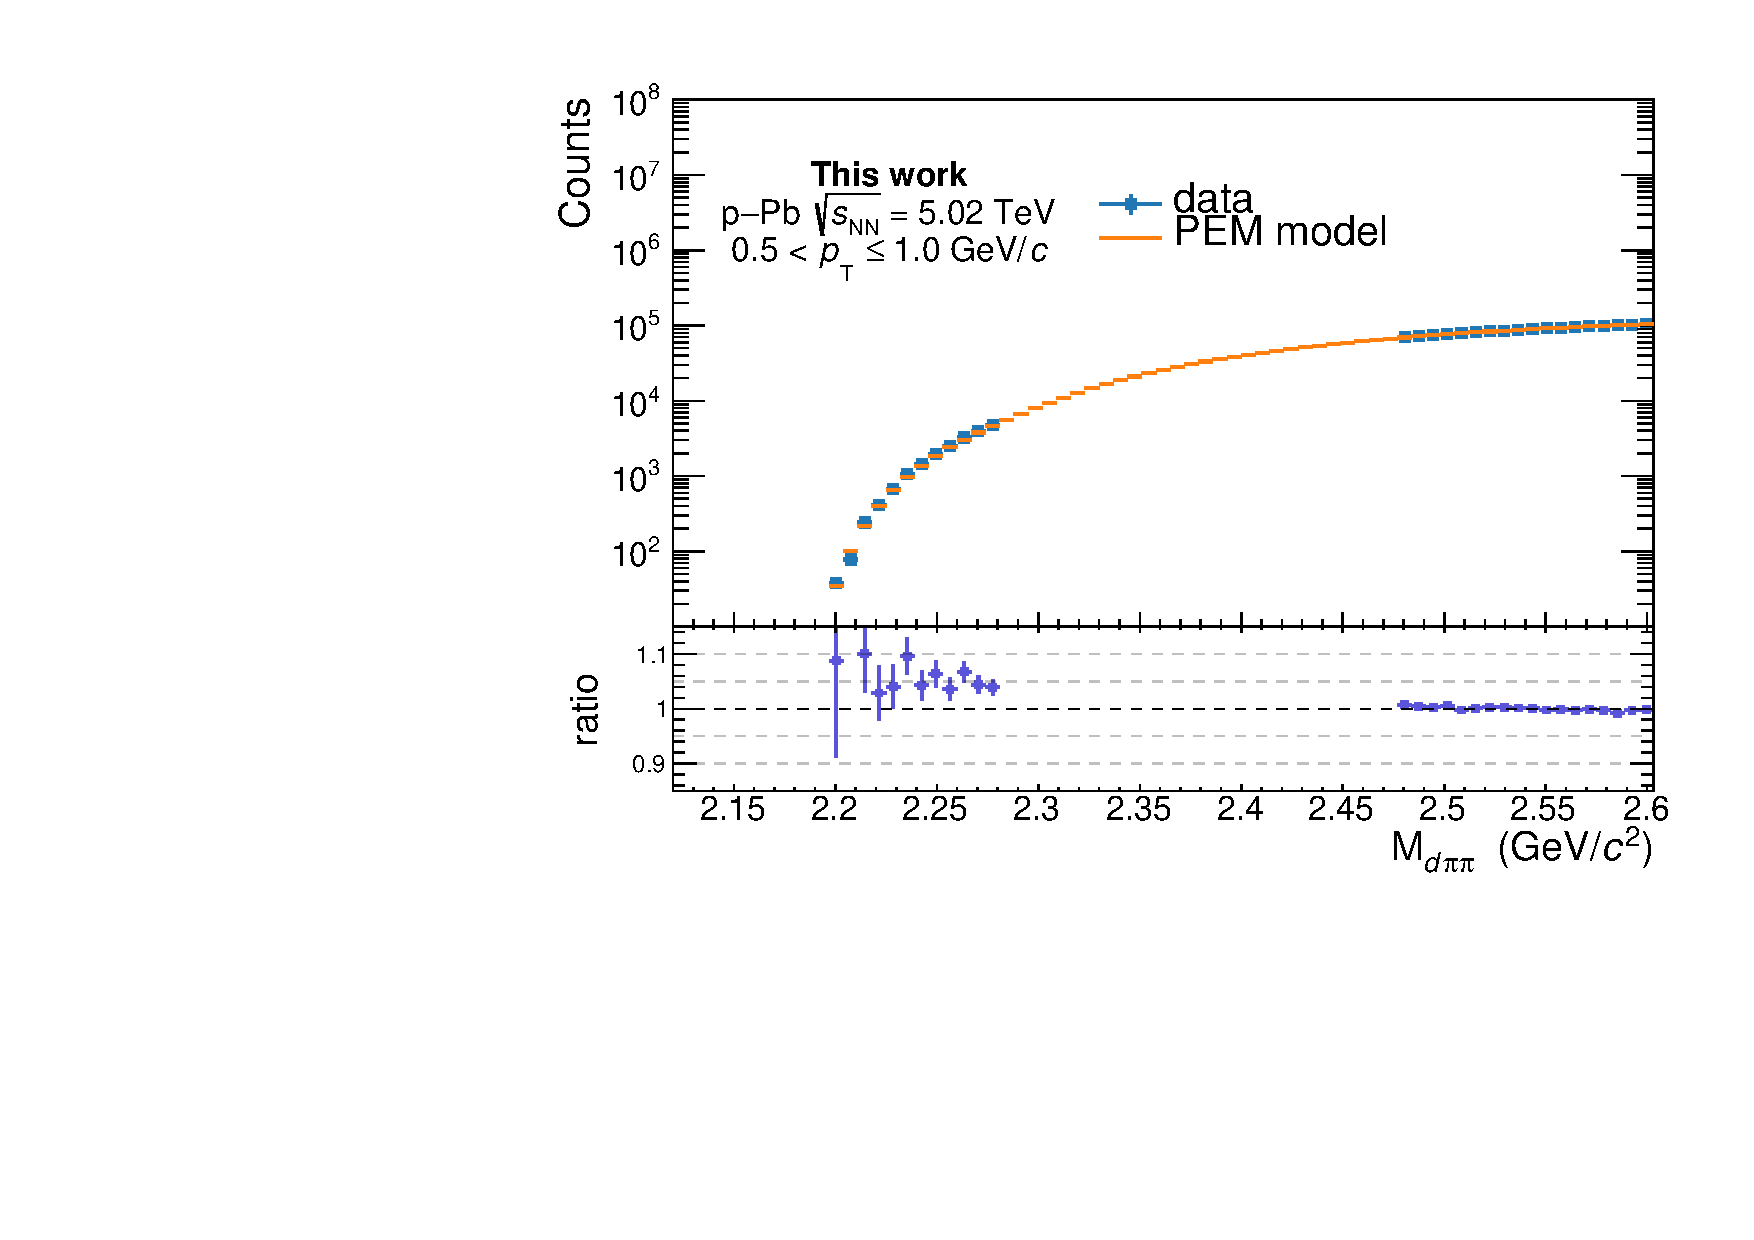
\includegraphics[width=0.75\textwidth]{gfx/appendix/pem/can_blindPEM1}
    \caption{PEM model compared with \minv, in the $0.5 < \pt \leq 1.0$ \gevc interval, outside the region of interest. In the lower pad the data/model ratio is reported.}
    \label{fig:pem05-1}
\end{figure}

The normalisation of the PEM model to the data has been done in the interval from 2.480 to
2.600 \gevcs. Smaller intervals have been studied, but the final findings do not
change in any meaningful way. The normalisation has not been performed in the region on the left 
of RoI because the model does not well describe the data in that region.

The PEM model can reproduce quite well the data in the region on the right of the RoI,
particularly for $\pt < 1.0\ \gevc$. In this region the difference between
data and model is < 2\%, but a trend is clearly visible in the ratio.
This trend is bigger for $\pt > 2.0\ \gevc$.
Instead the left sideband is not well reproduced by this model in all the considered \pt 
intervals. Figure~\ref{fig:pem05-1} shows the comparison between data \ -- with the region 
of interest blinded -- \ and the model in the \pt interval in which the description is
good. While Figure~\ref{fig:pem2-2.5} shows, as an example, the data-model comparison in the
$2.0 < \pt \leq 2.5\ \gevc$ interval in which the description is not satisfactory.
The data/model ratio is reported for both cases.

\begin{figure} [htb]
    \centering
    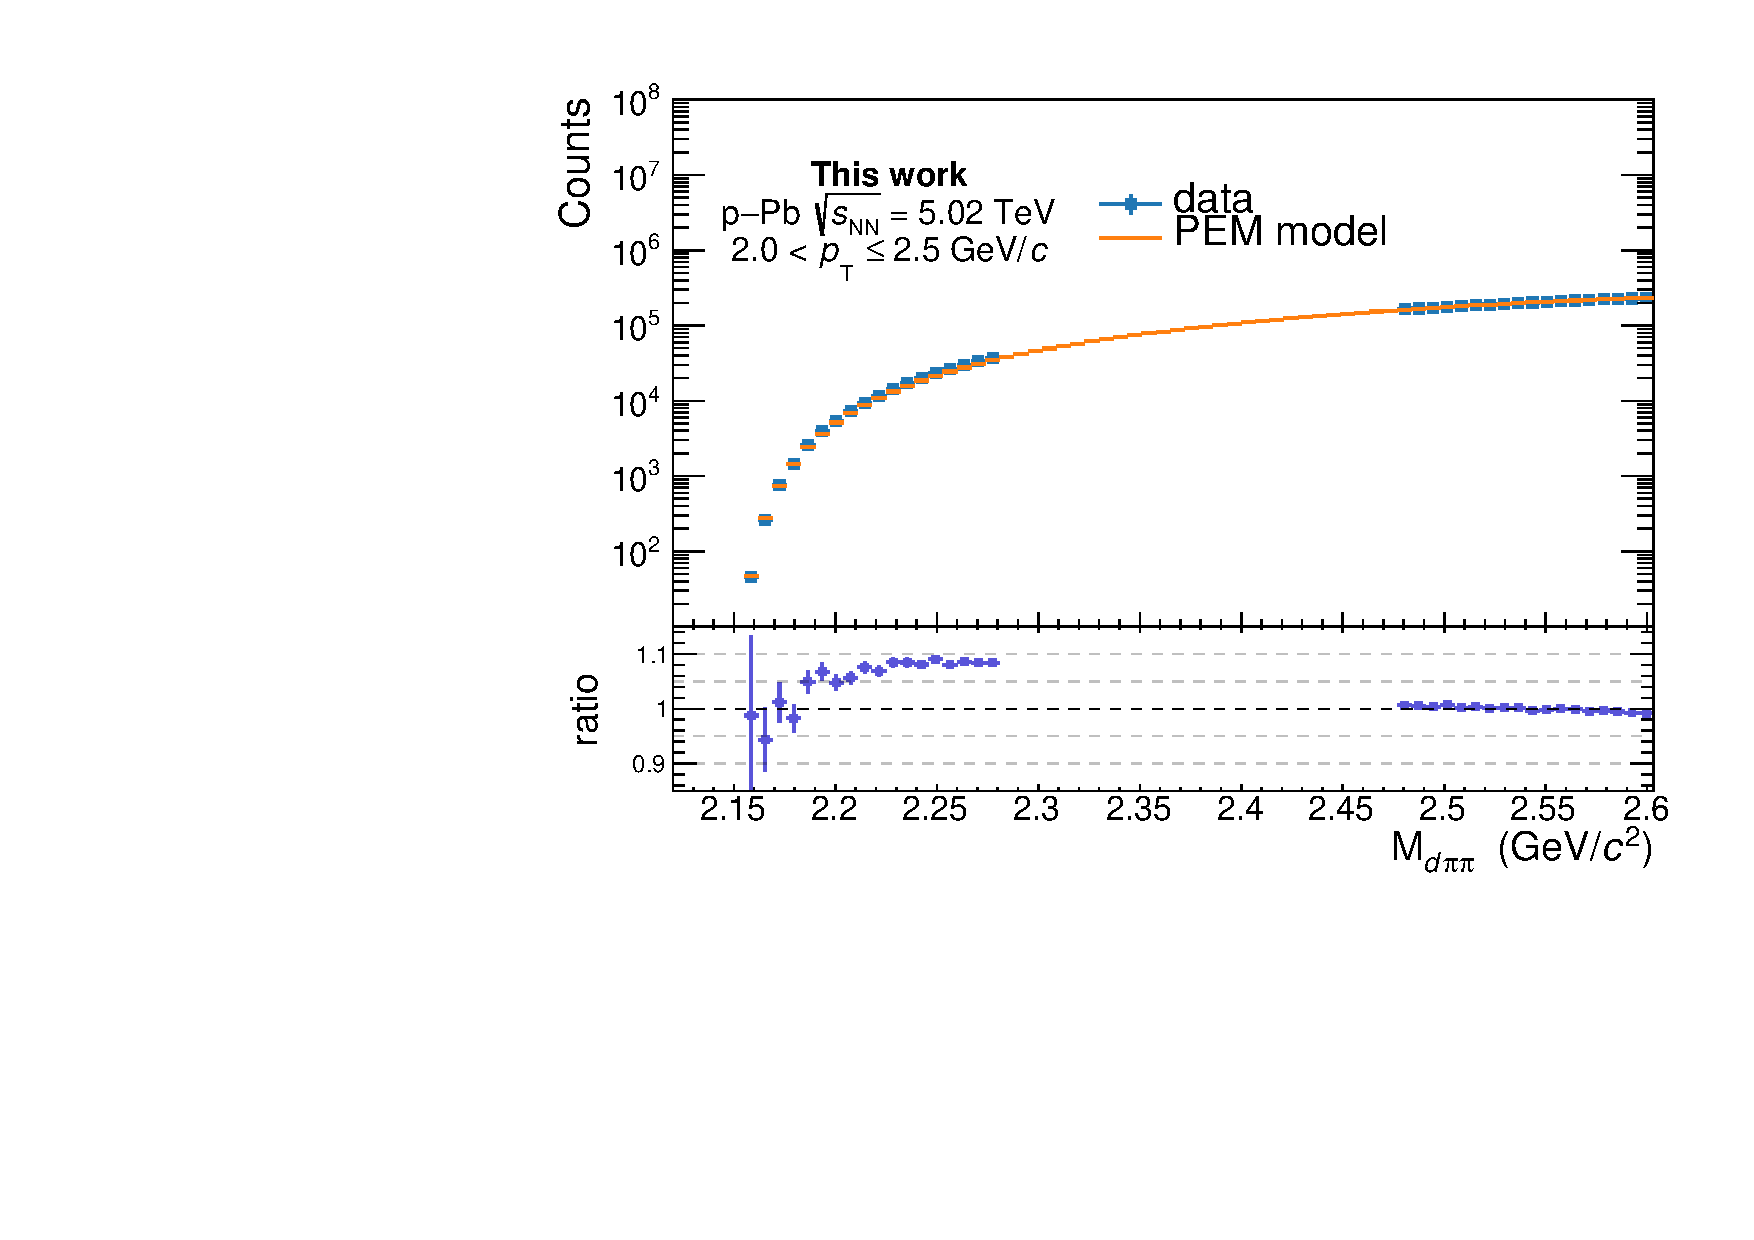
\includegraphics[width=0.75\textwidth]{gfx/appendix/pem/can_blindPEM4}
	\caption{PEM model compared with \minv, in the $2.0 < \pt \leq 2.5$ \gevc interval, outside the region of interest. In the lower pad the data/model ratio is reported.}
	\label{fig:pem2-2.5}
\end{figure}

The background description provided by the PEM model is not satisfactory in the whole \pt range
considered.
One can think that the discrepancies from data are due to some deuteron-pion correlation
that are not considered.

Therefore other two components of the PEM model have been derived mixing $d-\pip$ and
$d-\pim$ pairs from the same event and other pion from another event.
The resulting model is the weighted sum of the $\pi-\pi$, the $d-\pip$ and the $d-\pim$ components
of the PEM model.
The relative weights of the 3 contributions was found fitting the model to the data outside the RoI
with the relative weights as fit parameters and the sum of the weights constrained to be one.
This new model improves the background description.
In low \pt region \ -- $\pt < 1.5\ \gevc$ -- \ the data/model ratio is almost the same as in the case
of the previous model, while for higher \pt the discrepancies in the left sideband are < 5\%.
This value, compared with the previous 10\% of discrepancies shows that the new PEM
model provides a better background description: as an example 
Figures~\ref{fig:pemimp05-1} and~\ref{fig:pemimp2-2.5} show the data-model comparison in the same 
transverse momentum intervals reported in Figures~\ref{fig:pem05-1} and~\ref{fig:pemimp2-2.5}.

\begin{figure} [htb]
    \centering
    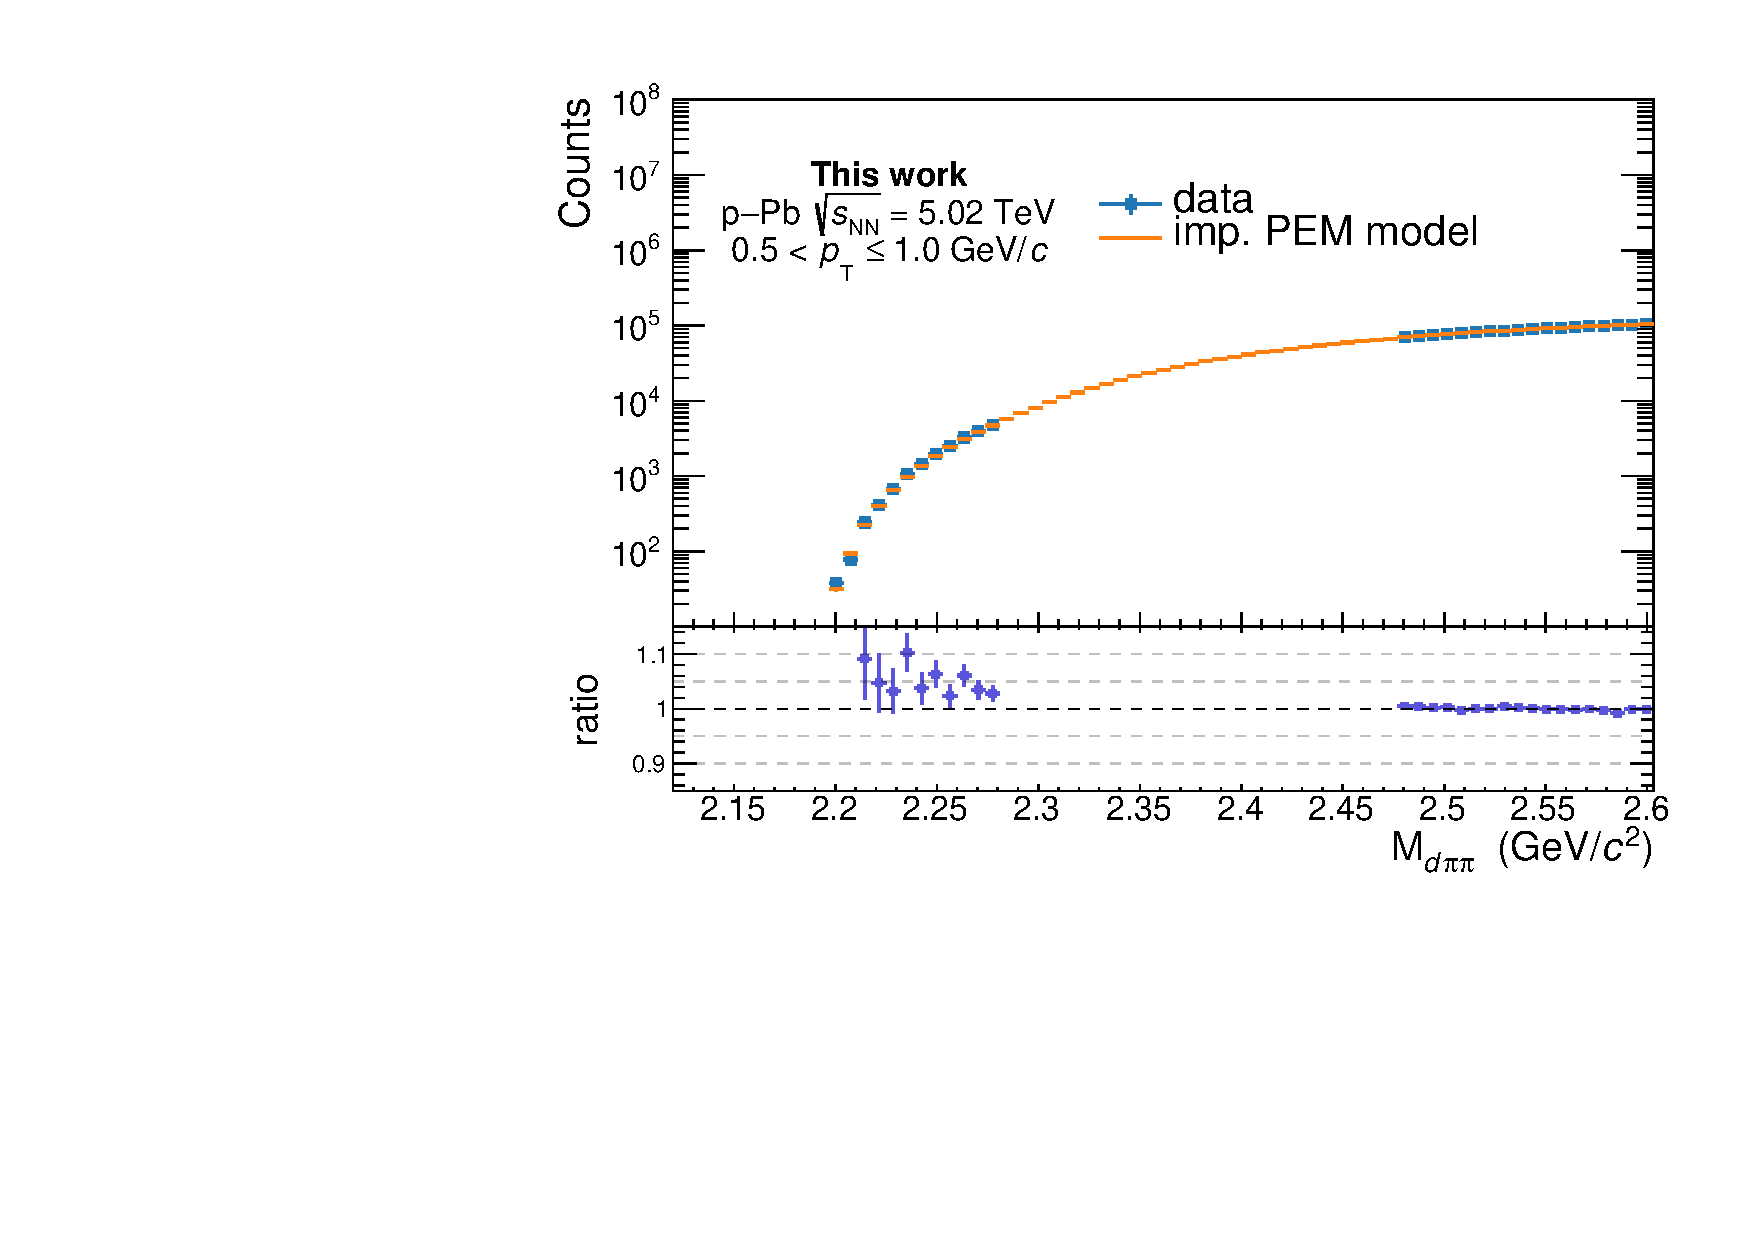
\includegraphics[width=0.75\textwidth]{gfx/appendix/impem/can_blindPEMimp1}
    \caption{Improved PEM model compared with \minv, in the $0.5 < \pt \leq 1.0$ \gevc interval, outside the region of interest. In the lower pad the data/model ratio is reported. In this \pt interval the description provided by the new model is not significantly better than the previous model one.}
    \label{fig:pemimp05-1}
\end{figure}
\begin{figure} [htb]
    \centering
    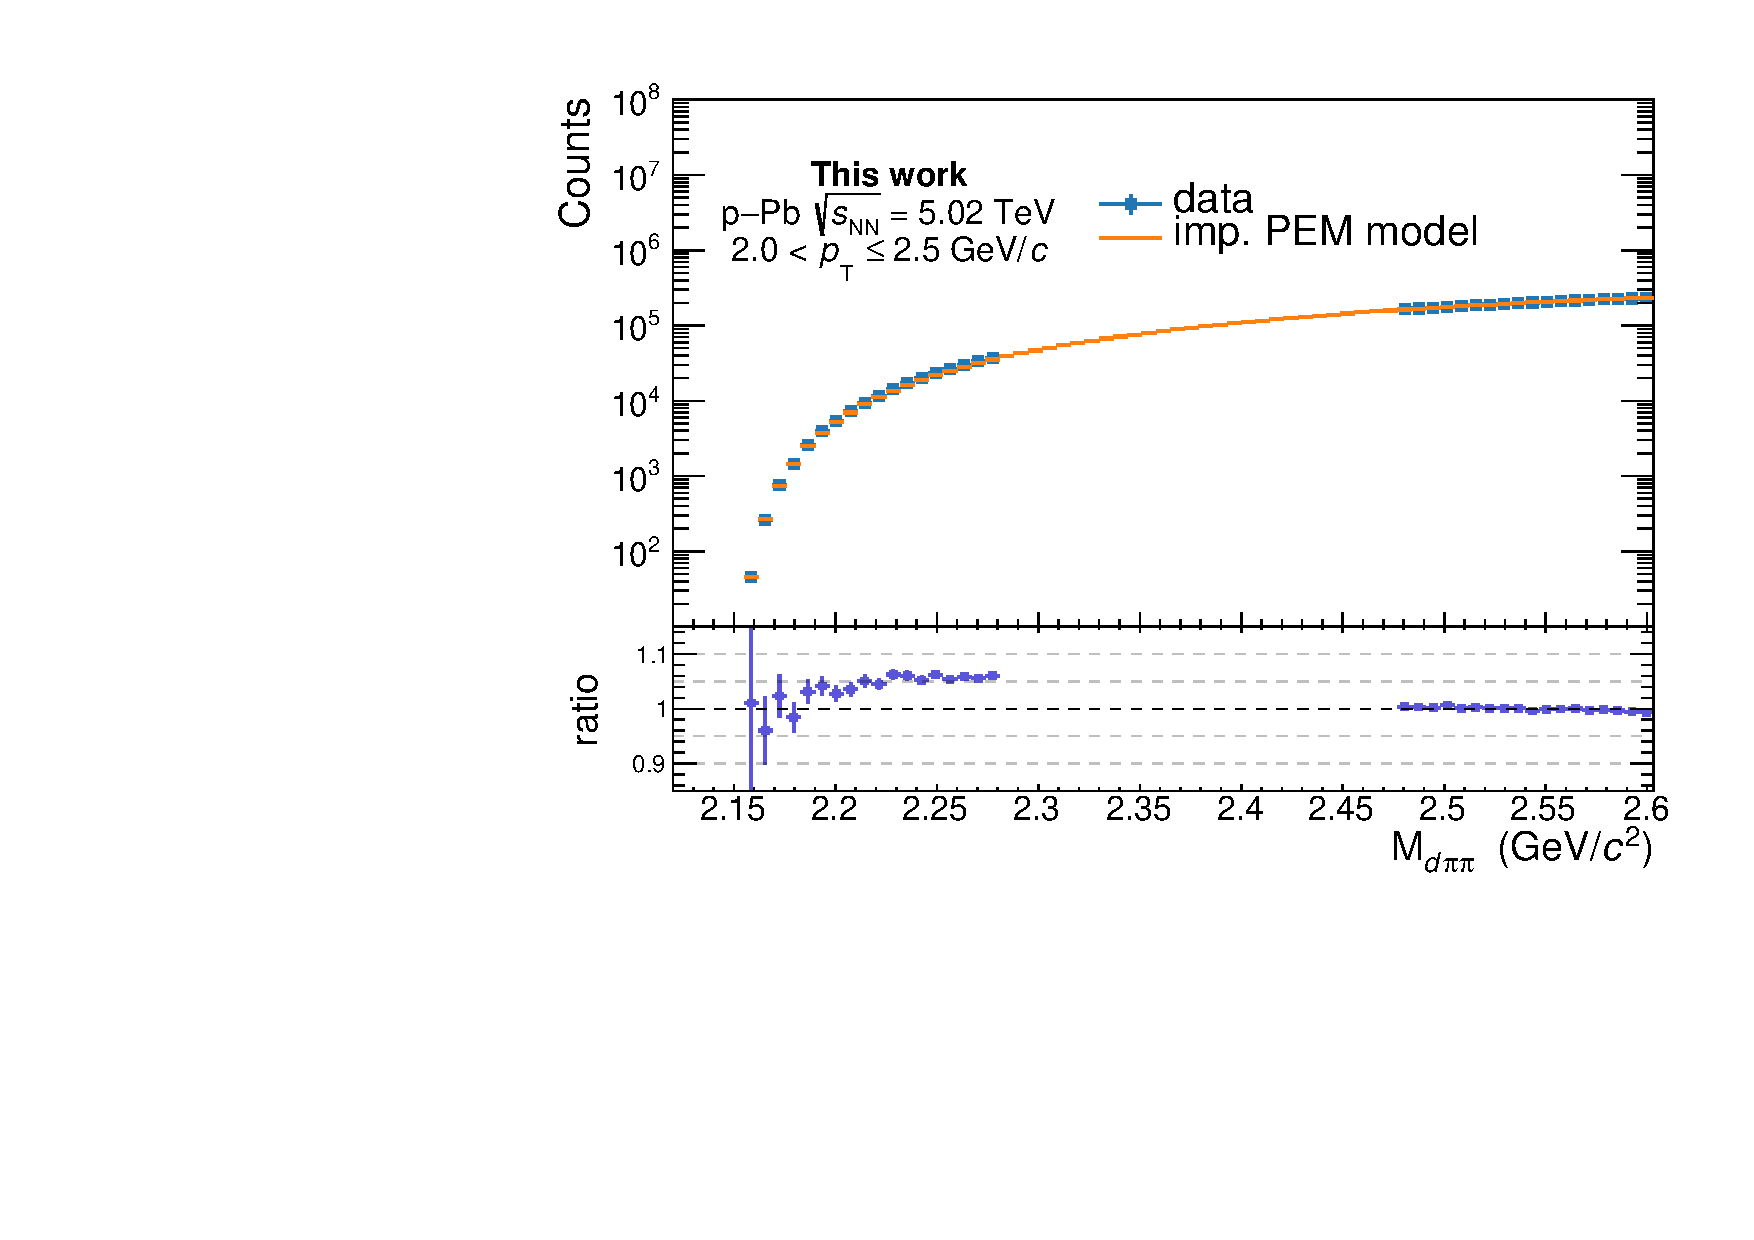
\includegraphics[width=0.75\textwidth]{gfx/appendix/impem/can_blindPEMimp4}
    \caption{Improved PEM model compared with \minv, in the $2.0 < \pt \leq 2.5$ \gevc interval, outside the region of interest. In the lower pad the data/model ratio is reported. In this \pt interval the new model improve the performances of the previous model, reducing the relative data-model discrepancies of a factor $\sim 2$.}
	\label{fig:pemimp2-2.5}
\end{figure}

The full list of figures related to the PEM and the improved PEM model as available in the 
appendix~\ref{app:pem} and~\ref{app:pemimp}.

%
\subsection{Template + Event Mixing model} \label{sec:tem}

The Template + Evnt Mixing model tries to reproduce the correlated backgrounds with a Monte Carlo
based template for each background component, while the uncorrelated background is described with a
real classical event mixing with all three tracks from three different events.

The templates are obtained combining deuterons from data \ -- to ensure that they have the correct
momentum spectrum -- \ with pion pairs from Monte Carlo data \ -- in order to have the information
about pion mothers.
In the Monte Carlo every reconstructed pion pairs has been considered.
Looking at the Monte Carlo truth of the pion mothers, the pion sources that provide pion pairs with 
mass, summed with deuteron mass, in 2.120 - 2.600 \gevcs range, has been estimated.
Then for each source the template was obtained combining pion pairs \ -- with the same mother imposed
-- \ with deuterons from the data. 
Basically each template is a \minv histogram with pion pairs from MC \ -- from the same mother and 
from the same source -- \ and deuterons from data. 
Each pion pairs was mixed with 50 different deuterons in the same $z_{vertex}$ class in order to 
increase the statistics of the templates.

This process has been done for the three \pt intervals considered, obtaining different templates in 
each \pt bin.
The remaining background, which should be now totally uncorrelated, is described with a real event 
mixing, obtained combining all three tracks from data from three different events in the same 
$z_{vertex}$ class.
Templates have been derived for sources with a contribution to the background at least of $10^{-4}$ of
the total in each \pt bin:
\begin{itemize}
  \item[] 0 -- 1 \gevc $\rightarrow \ \omega(782),\ \eta,\ \mathrm K_{0}^{S},\ \eta^{'}(958),\ \gamma $
  \item[] 1 -- 2 \gevc $\rightarrow \ \omega(782),\ \eta,\ \mathrm K_{0}^{S},\ \eta^{'}(958),\ \gamma $
  \item[] 2 -- 3 \gevc $\rightarrow \ \omega(782),\ \eta,\ \eta^{'}(958),\ \mathrm K_{0}^{S},\ \phi(1020),\ \gamma $
\end{itemize}

In each \pt bin the TEM model has been obtained as the weighted sum of the templates and the
uncorrelated component, where the weights are the fractions with which each template contributes to
the total background.
The weights were estimated starting from the abundance of each background source considered in the MC
production.
Of course there is a degree of uncertainty on the MC abundances, therefore the models has been fitted
to the data in each
\pt bin with weights as fit parameters. The weights has been constrained to be in $\pm$10\% range of 
the MC estimated value.

\begin{figure} [htb]
\begin{subfigure}{.33\textwidth}
  \centering
  \captionsetup{justification=centering}
  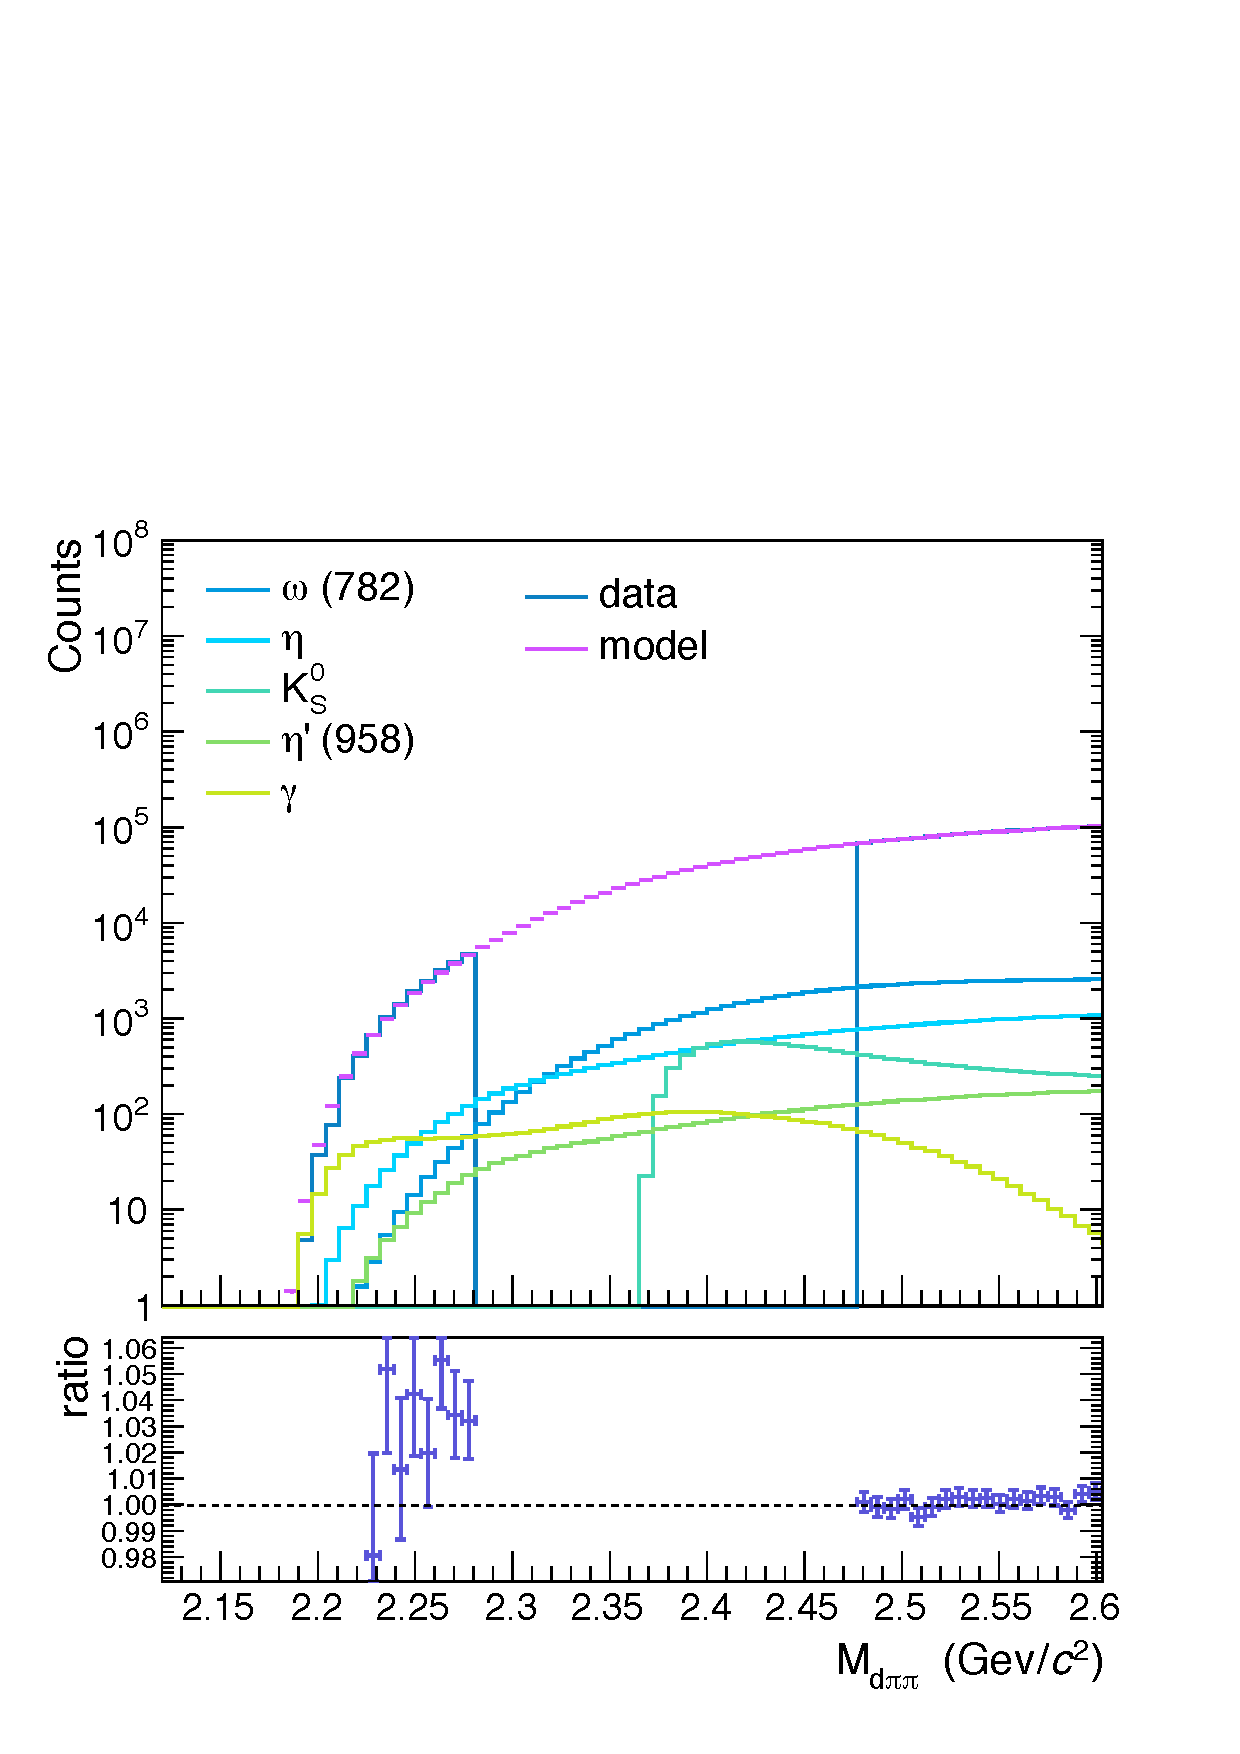
\includegraphics[width=\linewidth]{gfx/can0}
  \caption{}
  \label{fig:tem01}
\end{subfigure}%
\begin{subfigure}{.33\textwidth}
  \centering
  \captionsetup{justification=centering}
  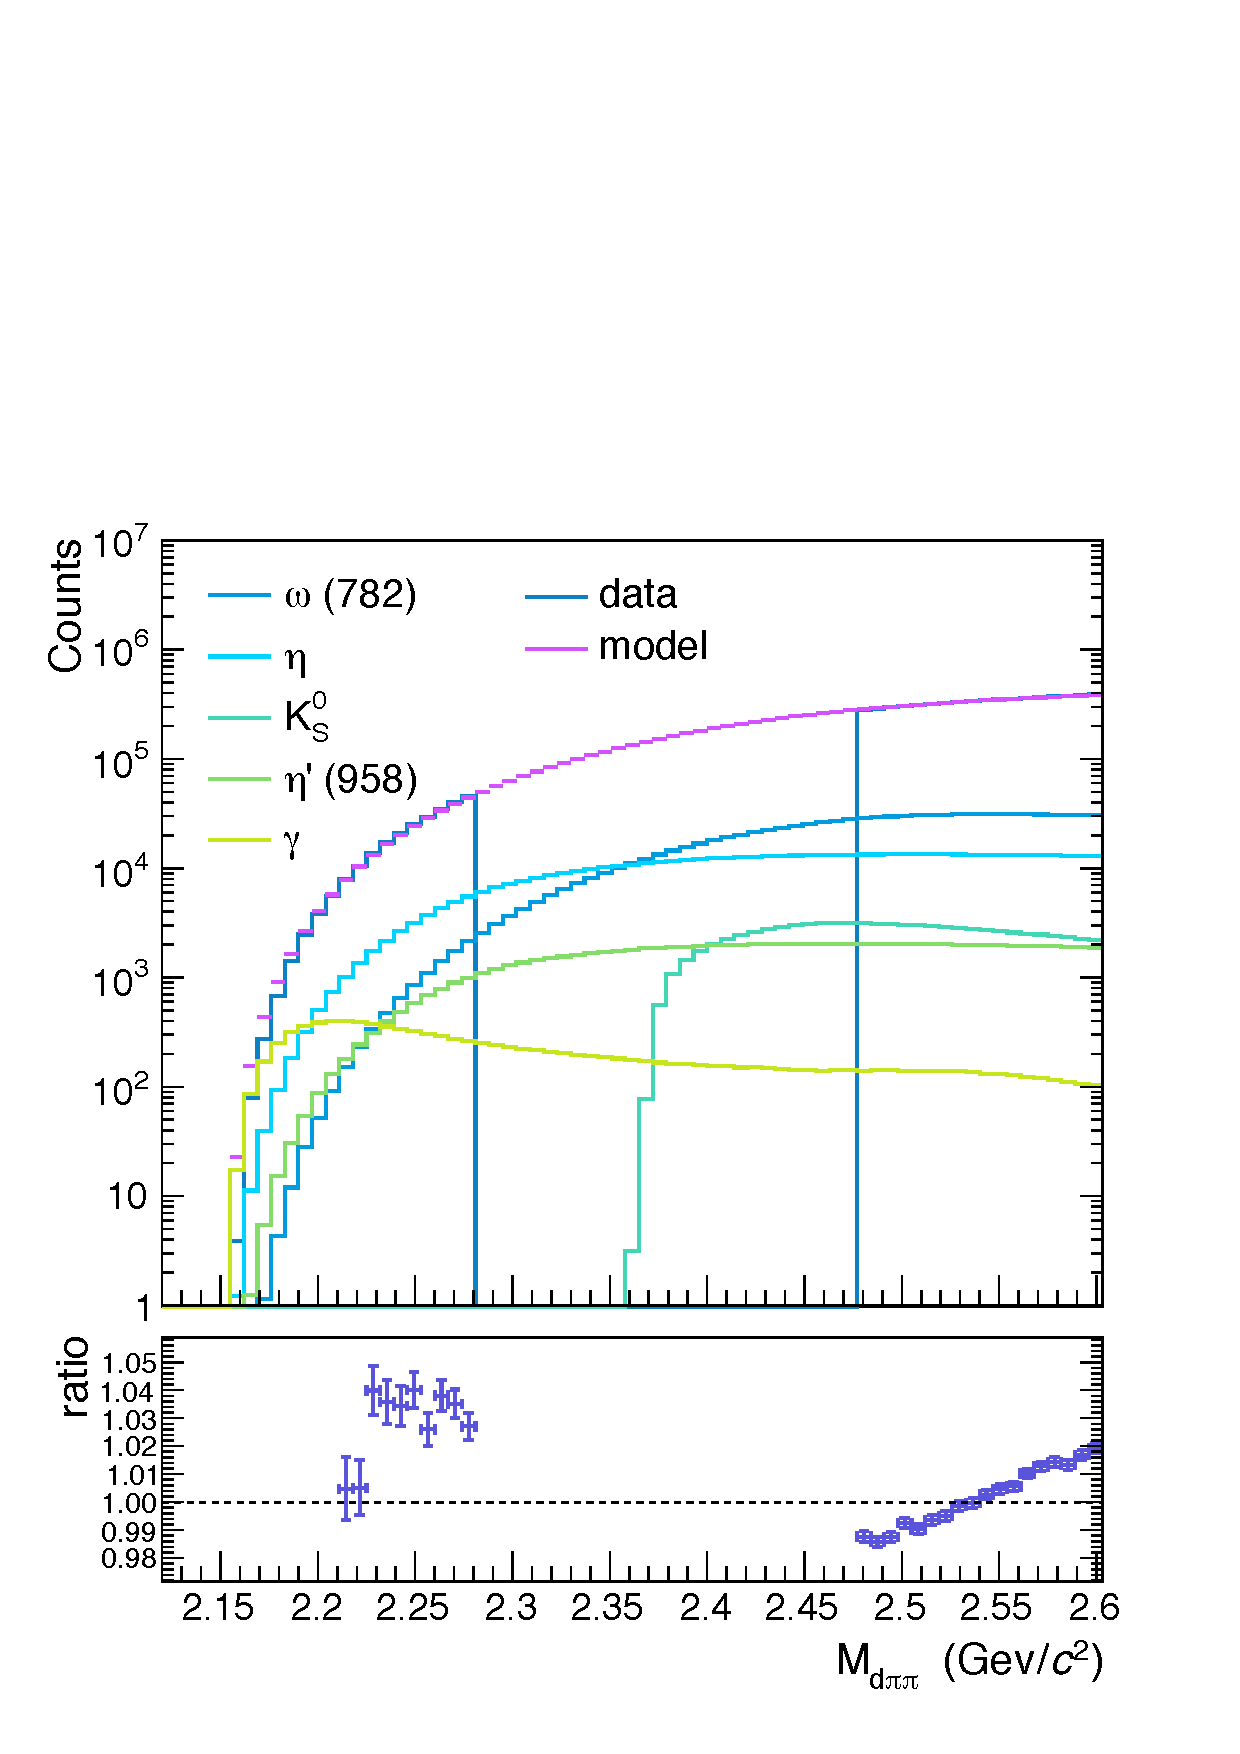
\includegraphics[width=\linewidth]{gfx/can1}
  \caption{}
  \label{fig:tem12}
\end{subfigure}
\begin{subfigure}{.33\textwidth}
  \centering
  \captionsetup{justification=centering}
  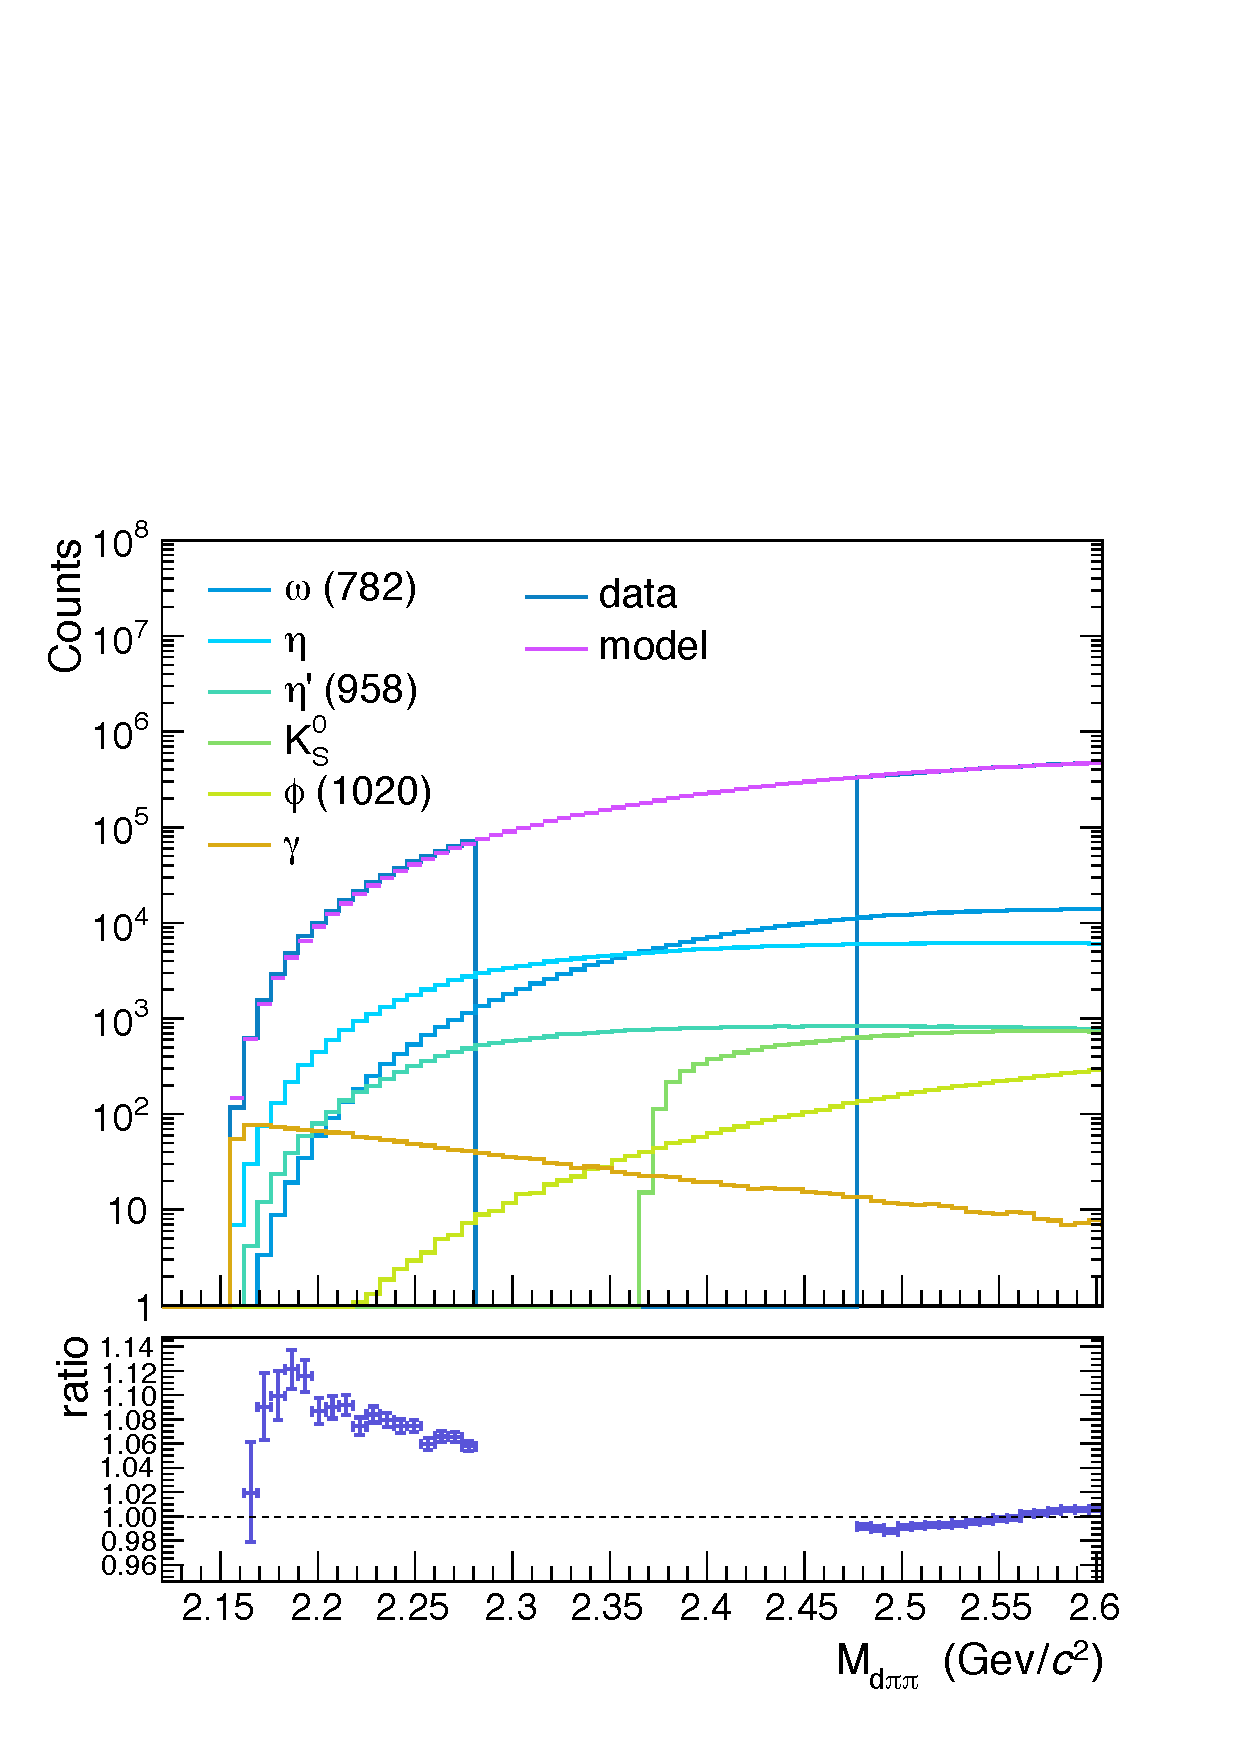
\includegraphics[width=\linewidth]{gfx/can2}
  \caption{}
  \label{fig:tem23}
\end{subfigure}
\caption{The TEM model (magenta line) is compared with \minv from data (blue line) in 0 - 1 \gevc transverse momentum interval. The other lines represent different templates that contribute to the TEM model.}
\label{fig:tem01}
\end{figure}

The TEM model provides a better background description then PEM model. In the first \pt bin
(Fig.~\ref{fig:tem01}) the data/model ratio is flat in the right sideband, while in the left sideband 
discrepancies are around 3\%. In the second bin (Fig.~\ref{fig:tem12}) the situation is a little worse
with a linear trend in the data/model ratio visible in the right sideband \ -- differences from flat
ratio < 2\% -- \ while in the left sideband the description is similar to that from the first bin. 
In the last considered bin (Fig.~\ref{fig:tem23}) the description get worse, in the right sideband
there is a linear trend similar to the one observed in the second bin, while in the left sideband 
discrepancies from flat ratio are around 8-10\%.

The TEM model provides, not only a better background description, but also an estimation of
the background sources and the shapes of their contribution to the total background.

Except for the $K_{s}^{0}$ meson, the templates show a smooth shape, so it is expected that they do 
not give rise to suspicious structures in the RoI. The situation is different for the $K_{s}^{0}$ 
which template has the kinematic limit just where the \ds is expected to be.
This can be a problem, but we can set the weight of the $K_{s}^{0}$ template measuring his production
in the $\pip+\pim$ invariant mass distribution.

%
%
\section{Significance of the measurement} \label{sec:significance}

Before to perform the background subtraction to look for the \ds signal, the statistical significance
of the measurement has been estimated.
Three ingredients are needed to get the estimation of the significance: the expected signal shape, 
a plausible background shape and normalisation and finally an the \ds yield.

In the previous sections the expected signal shape (Sec.~\ref{}) and the background shape (Sec~\ref{})
have been discussed. 
In this section the estimation of the expected \ds yield in \pPb collisions at \sctev \ -- based on the
Statistical Hadronization Model -- \ and finally, the estimation of the significance, is presented.

%
\subsection{Production yield estimation} \label{sec:ds_production}

In the Statistical Hadronization Model framework, described in Section~\ref{sec:1.4.1}, is possible 
to estimate the expected production yield of the \ds. Following equation~\eqref{eq:particleyields1}
the average particle yield for a species $i$ is related to the mass of the specie itself by the 
following relation:
\begin{equation} \label{eq:tm_prod1}
    \langle N_{i} \rangle \propto g_{i} e^{\beta m_{i}},
\end{equation}
where $\beta$ is the inverse of the chemical freeze-out temperature ($\beta = 1/T_{ch}$) and 
$g_{i}\ $ is the degree of degeneracy of the $i\ $ state. 
Therefore, using Equation~\eqref{eq:tm_prod1} the \ds/d ratio can be expressed as:
\begin{equation} \label{eq:tm_prod2}
\frac{\langle N_{\ds} \rangle}{\langle N_d \rangle}=\frac{g_{\ds}}{g_d}e^{-\beta (m_{\ds} - m_d)}=\frac{7}{3}e^{-\beta (m_{\ds} - m_d)}.
\end{equation}
In the range of chemical freeze-out temperature that typically describe nuclei production in
heavy ion collisions (between 155 and 170 MeV), the ratio is approximately $0.1$.
In order to compute the expected abundance of \ds in the 2016 \pPb data, an additional 
$0.22$ factor has to be applied to keep into account the branching ratio of the \dstdecay
decay channel under study.

The rate of expected \dstdecay in p–Pb inelastic collisions at \sctev is then 
approximately $2.46\times10^{-5}$ with an uncertainty of $14\%\ $ due to the $T_{ch}$
range assumed in the calculations. The value of the deuteron yield used to compute the \ds/d
ratio has been measured by the ALICE collaboration~\cite{deuteron_in_progress}.

%
\subsection{Significance estimation} \label{sec:sig_sub}

While the signal shape has been obtained by reconstructing true \ds candidates in the Monte Carlo~\ref{sec:4.2.1},
the background shape and normalisation was extracted by studying the like sign triplets in the data
\ -- $\ds \rightarrow d+\pip+\pip$  and $\ds \rightarrow d+\pim+\pim$ and their respective charge conjugate). 
As \ds yield has been considered the thermal model estimations presented in Section~\ref{sec:ds_production}.

\begin{figure} [htb]
\centering
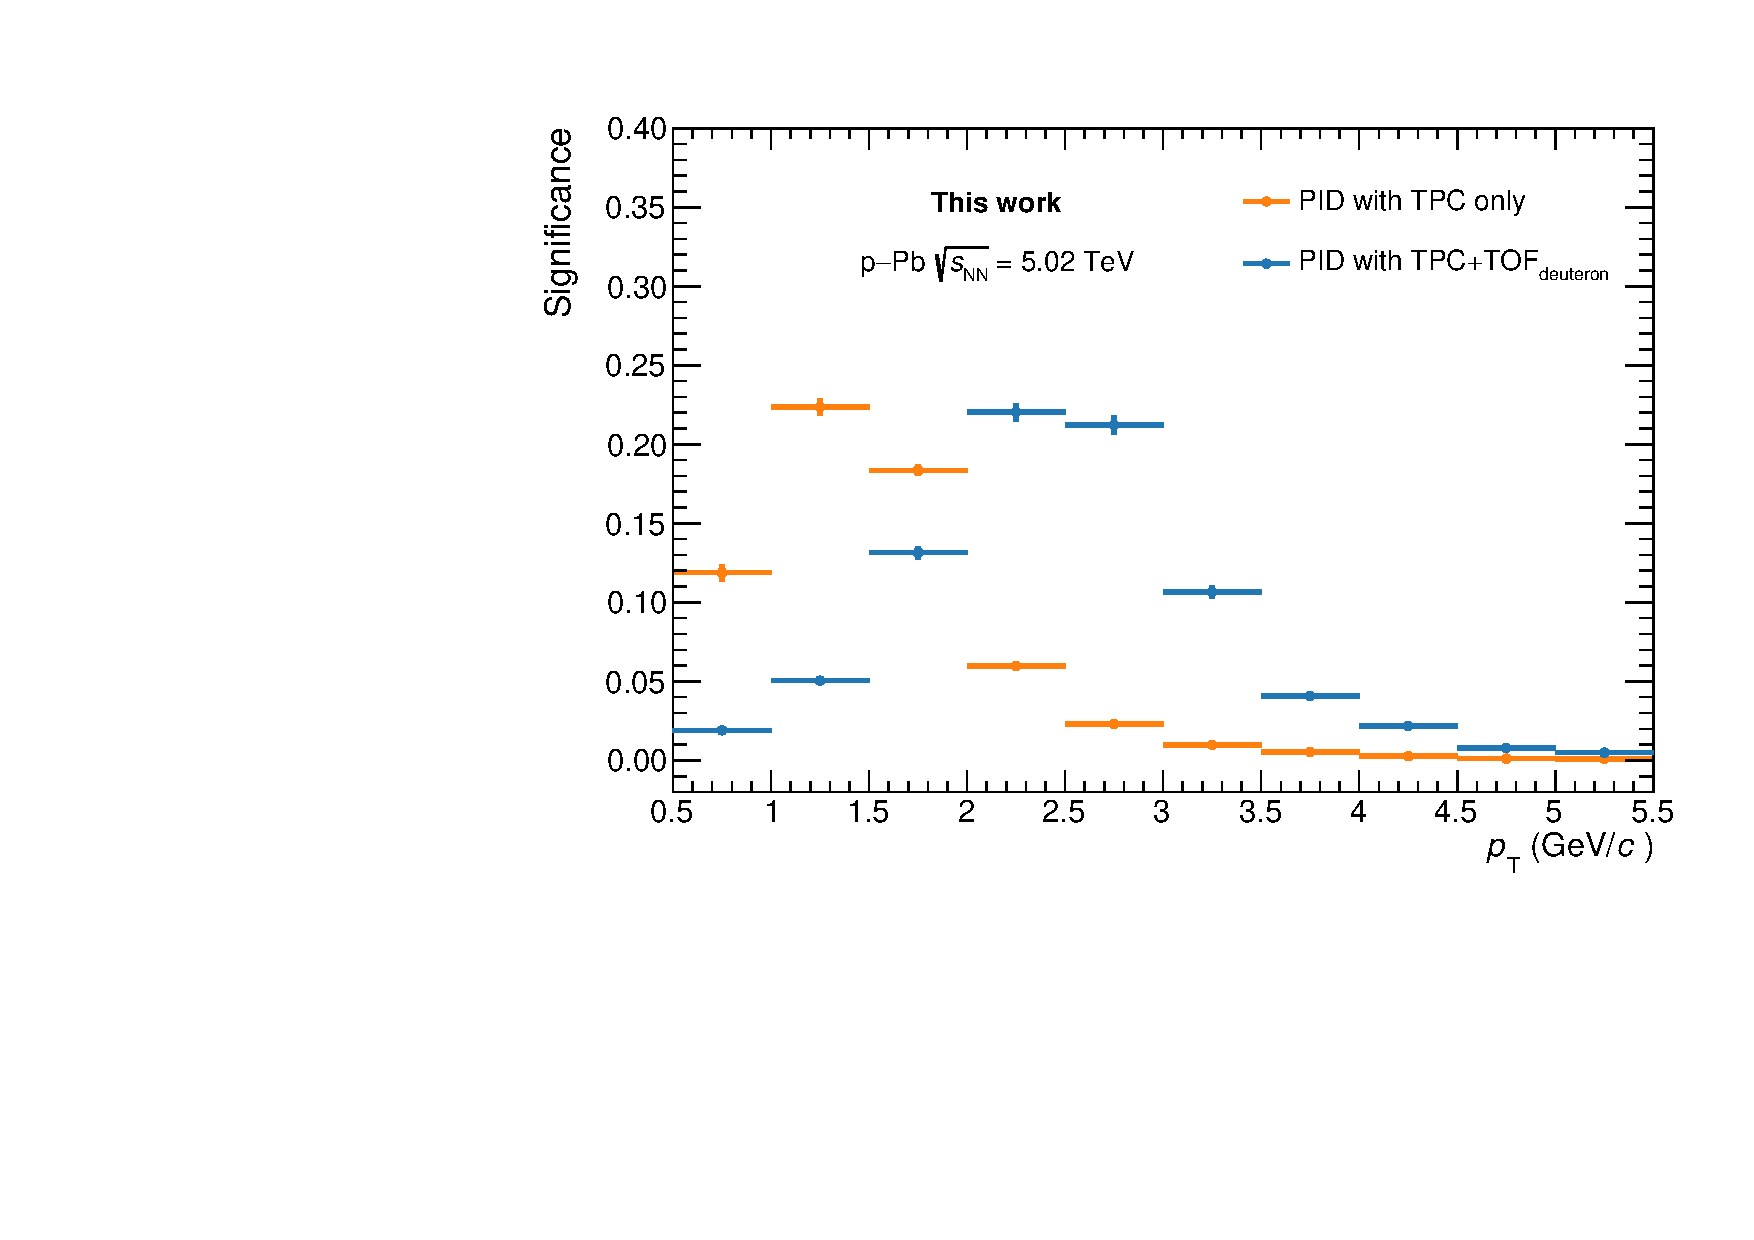
\includegraphics[width=0.7\linewidth]{gfx/sigcomp}
\caption{Significance of the measurement as a function of transverse momentum compared for the TPC and the TPC+TOF$_{deuteron}$ PID configurations.}
\label{fig:significance}
\end{figure}

The significance has been estimated by integrating signal and background in a 70 \mevcs wide region around the
expected mass peak of the \ds. 
Figure~\ref{fig:significance} shows the significance in various \pt bins for both the TPC and the
TPC+TOF$_{deuteron}$ PID configurations.
The first transverse momentum bin has been missed because the number of expected \ds correctly reconstructed 
in this interval is negligible with respect to the background.

While in the $0.5 \leq \pt \leq 2.0\ \gevc$ interval the TPC only PID guarantees an optimal identification of 
pions and deuterons showing the maximum of significance, starting from  $2.0\ \gevc$ the TPC+TOF$_{deuteron}$ 
configuration reduces the combinatorial background and improves the significance. 
The wide peak of the \ds makes its identification challenging for the experimental condition at the LHC and 
if the thermal model prediction is correct it is possible to set only an upper limit to the production yield
of \ds.

In the light of this study of the significance, the optimal choice of the PID configuration is to use the TPC
configuration for \ds candidate up to $2.0\ \gevc$ of transverse momentum, while to use the the TPC+TOF$_{deuteron}$
fot \ds candidate with transverse momentum $\geq 2.0\ \gevc$.

%
%
\section{Background subtraction} \label{sec:backsub}

After the estimation of the significance and a detailed study of the background of the measurement,
the region of interest has been \textit{unblinded} to look for the \ds signal.
Firstly, the the improved PEM model \ -- described in Section~\ref{sec:pem} -- \ has been compared
with the data in the region of interest, and the data/model ratio has been computed.

\begin{figure} [htb]
    \centering
    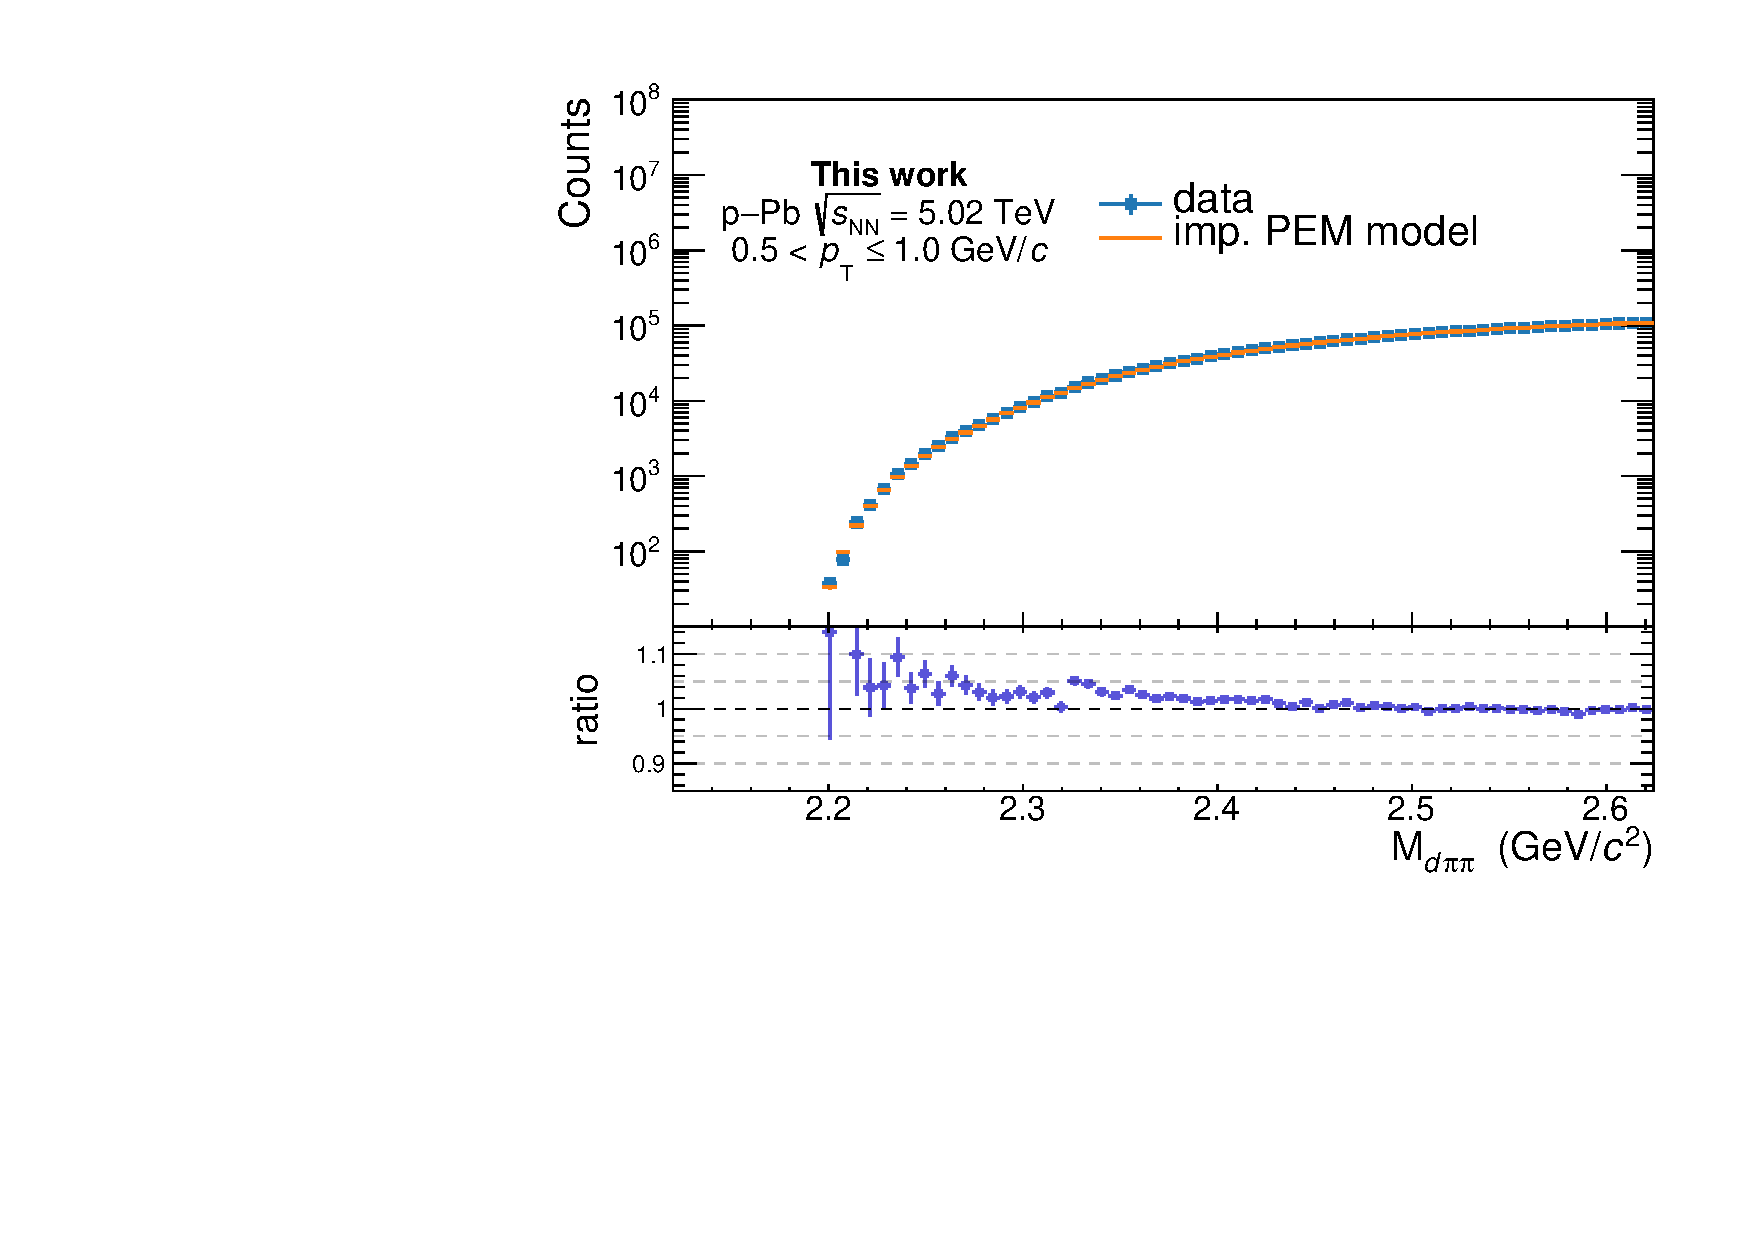
\includegraphics[width=0.75\textwidth]{gfx/appendix/backsub/can_unblind1}
    \caption{Improved PEM model compared with \minv, in the $0.5 < \pt \leq 1.0$ \gevc interval. In the lower pad the data/model ratio is reported.}
    \label{fig:unbl05-1}
\end{figure}

The data/model ratio is not flat in the region of interest, however, this was expected because of the 
data-model discrepancies observed outside the RoI (Sec:~\ref{sec:pem}).
Nevertheless, the data/model ratio does not show any shape around $2.380\ \gevcs$ that can be referred 
to the \ds signal.

\begin{figure} [htb]
    \centering
    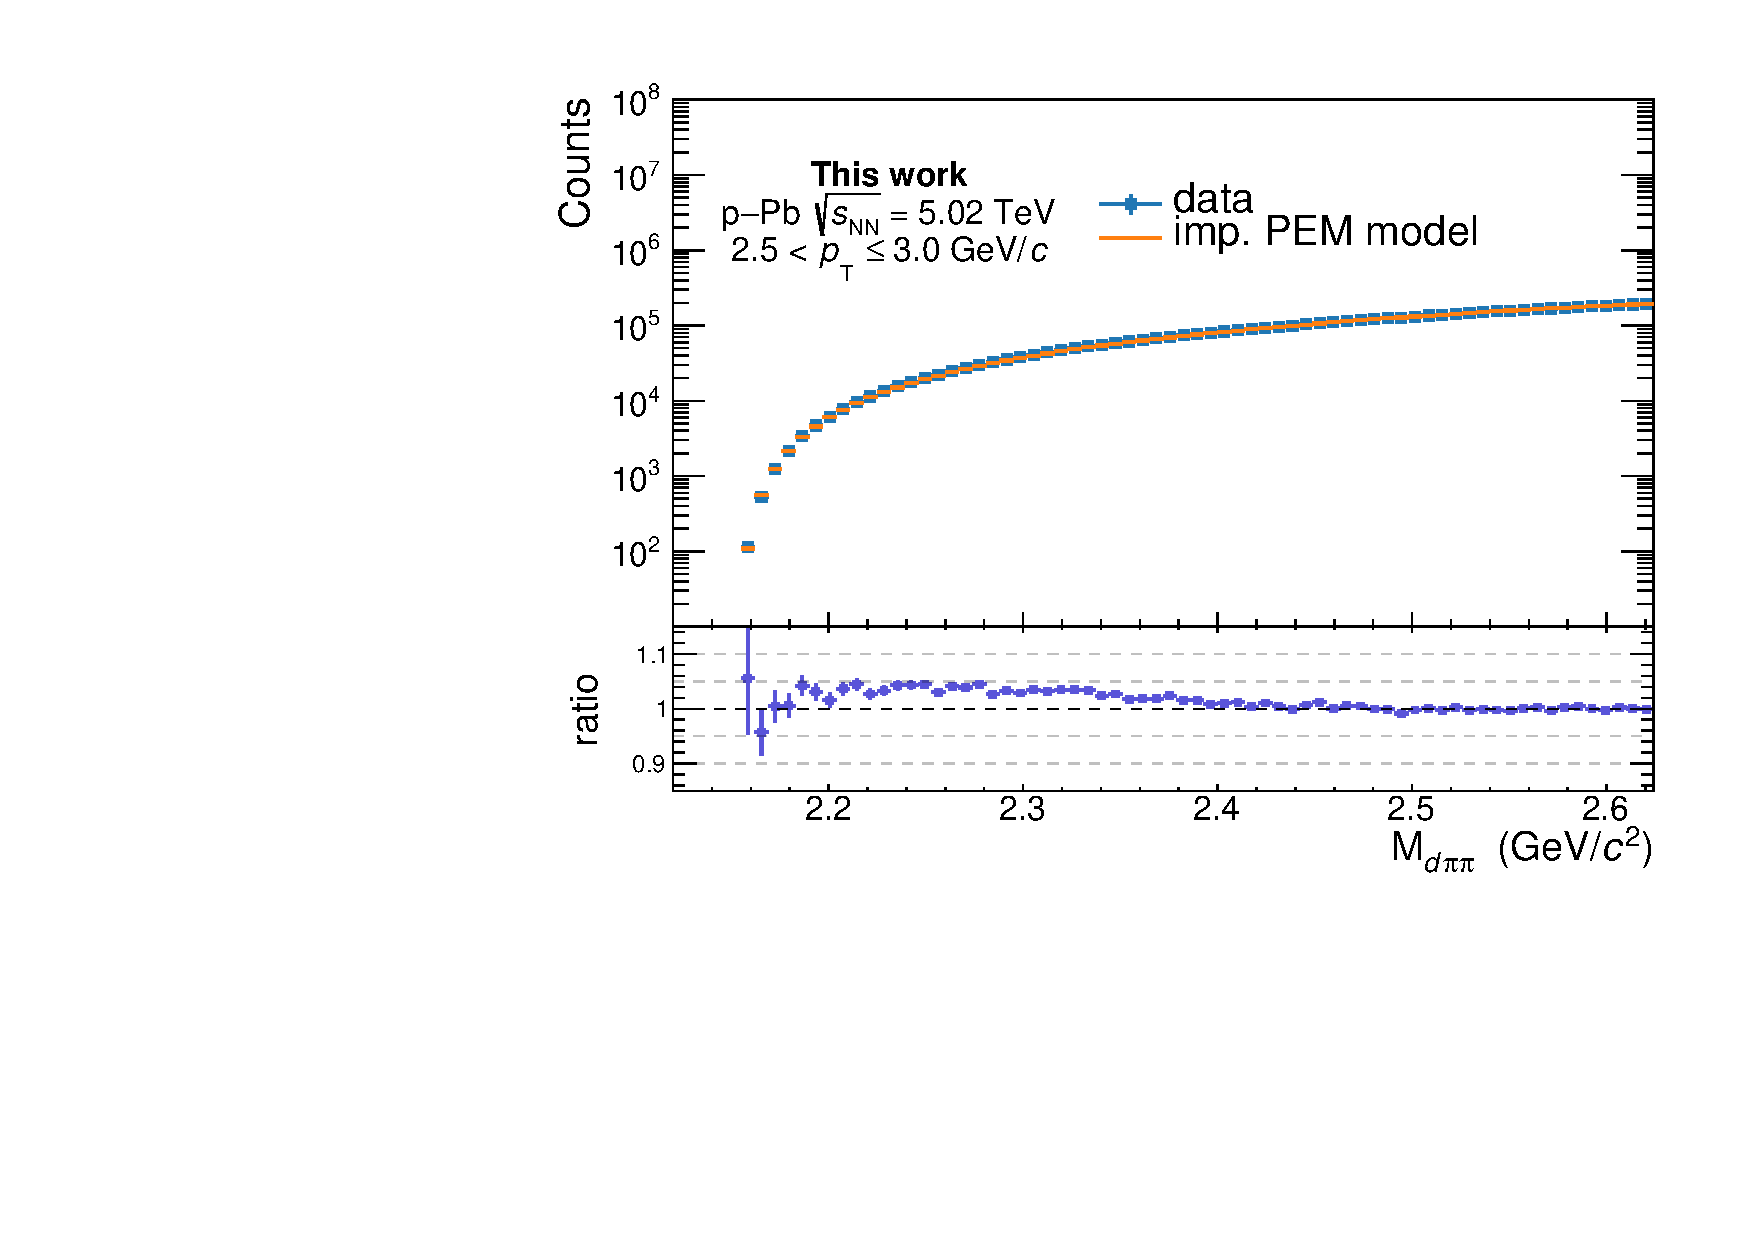
\includegraphics[width=0.75\textwidth]{gfx/appendix/backsub/can_unblind5}
    \caption{Improved PEM model compared with \minv, in the $2.5 < \pt \leq 3.0$ \gevc interval. In the lower pad the data/model ratio is reported.}
	\label{fig:unbl2.5-3}
\end{figure}

Figure~\ref{fig:unbl05-1} shows the comparison between data and model, in the region of interest,
in the transverse momentum interval in which the maximum of the production of the \ds is expected.
While Figure~\ref{fig:unbl2.5-3} shows the \pt interval in which the background description,
provided by the improved PEM model, is worst.
The data-model discrepancies reach a maximum of 5\% in the region of interest, which is in accordance 
with the maximum of 4\% outside the RoI shown in Figure~\ref{fig:pemimp2.5-3}.
The full list of figures related to this study is available in Appendix~\ref{app:bs1}.

Since there is no evidence of the presence of the \ds signal in the region of interest, it is possible
to assume that the data-model discrepancies are due to a background component that is not described by 
the model.
Therefore a gaussian component has been included in the improved PEM model in order to
reproduce the residual background.
The new background model \ -- i.e. improved PEM + gaussian component -- \ has been fitted to the data
outside the region of interest, in order to determine the gaussian parameters.
Then the model has been normalized to the data with the following normalizing constant:
\begin{equation}
    C = \frac{\int_{2.160}^{2.280}\mathrm{Data}(\minv) d\minv + \int_{2.480}^{2.620}\mathrm{Data}(\minv) d\minv}{\int_{2.160}^{2.280}\mathrm{Model}(\minv) d\minv + \int_{2.480}^{2.620}\mathrm{Model}(\minv) d\minv},
\end{equation}
% non è essenziale mettere la formula del fattore di normalizzazione, ma cosí è chiaro che cosa ho usato
% per normalizzare il modello ai dati
that ensure to not consider the signal region in the normalisation.
Finally the normalized model has been subtracted from the data. Figure 

\begin{figure} [htb]
    \centering
    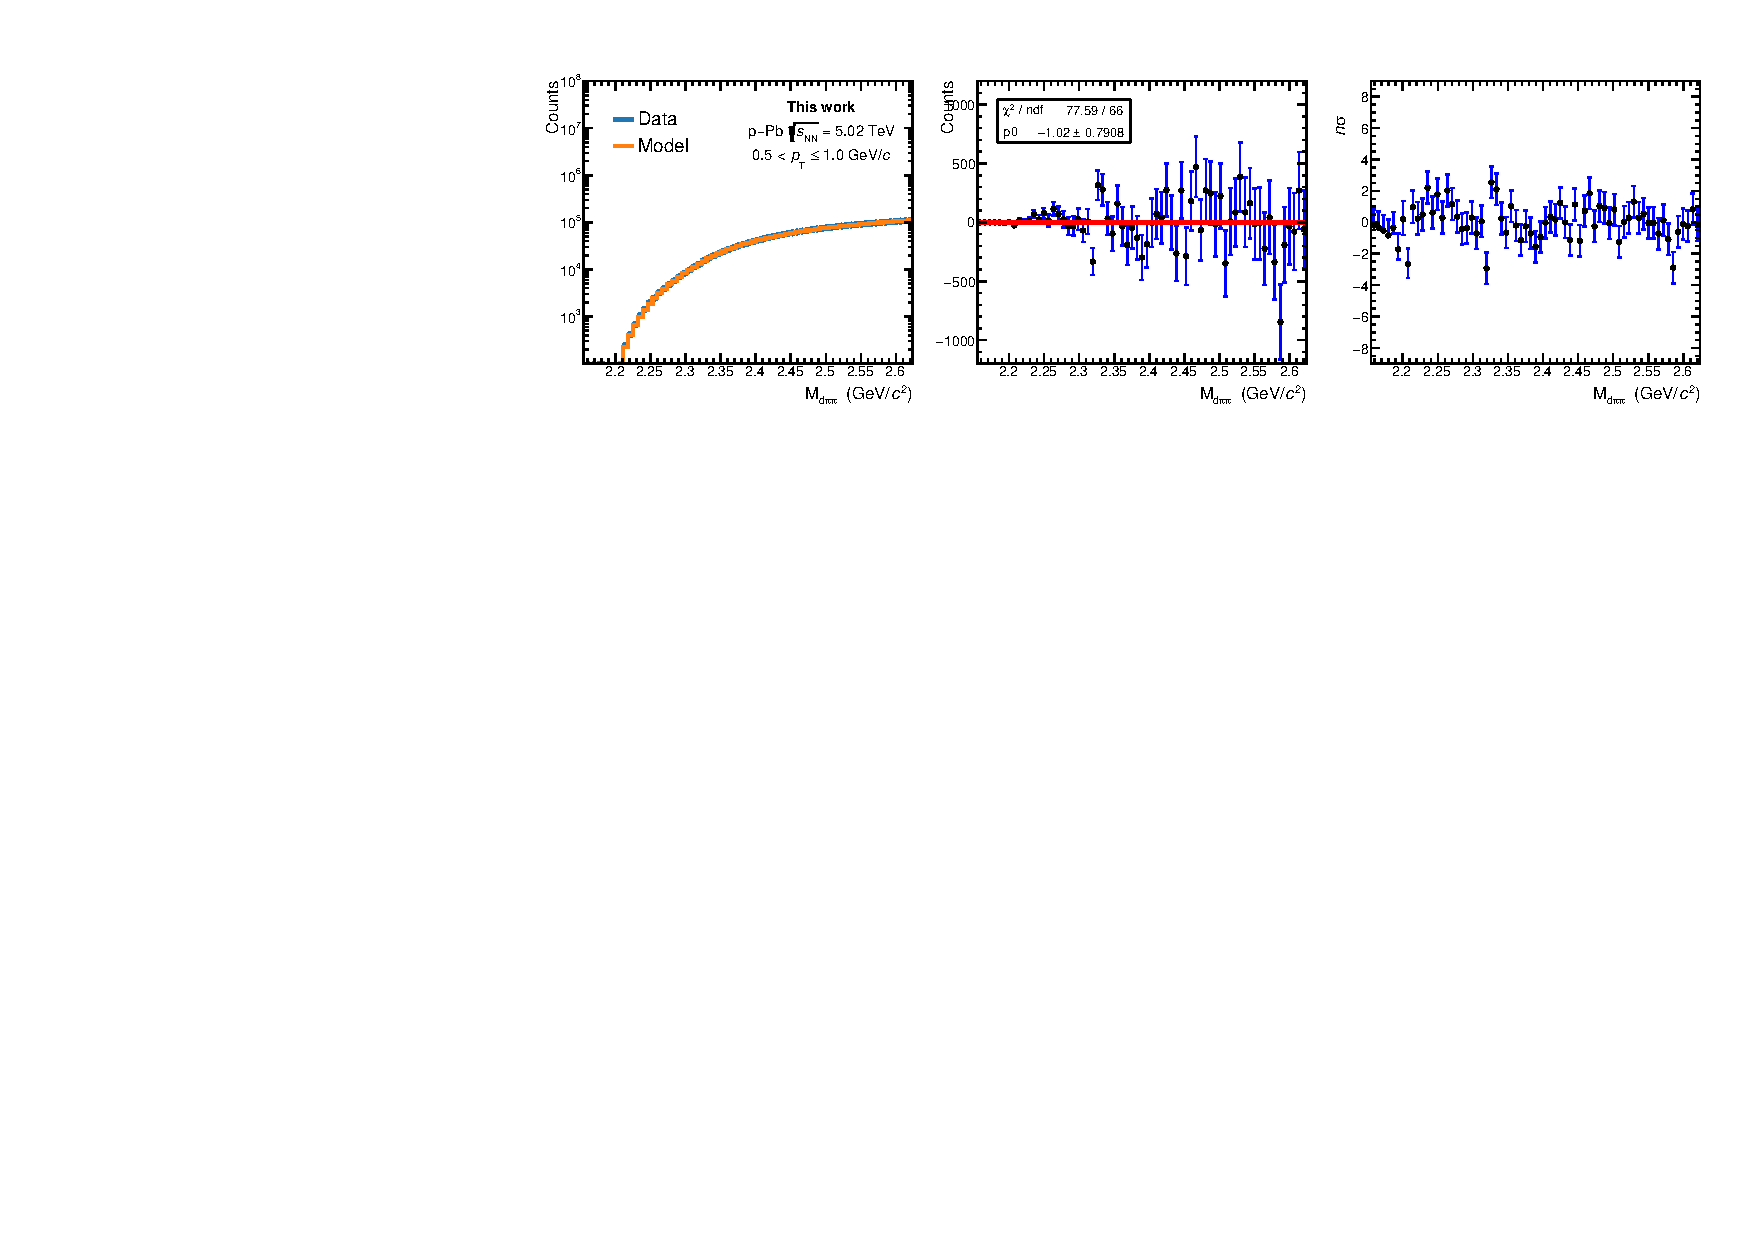
\includegraphics[width=\textwidth]{gfx/appendix/backsub/canvas1}
    \caption{Improved PEM model compared with \minv, in the $0.5 < \pt \leq 1.0$ \gevc interval. In the lower pad the data/model ratio is reported.}
    \label{fig:bs1}
\end{figure}

\begin{figure} [htb]
    \centering
    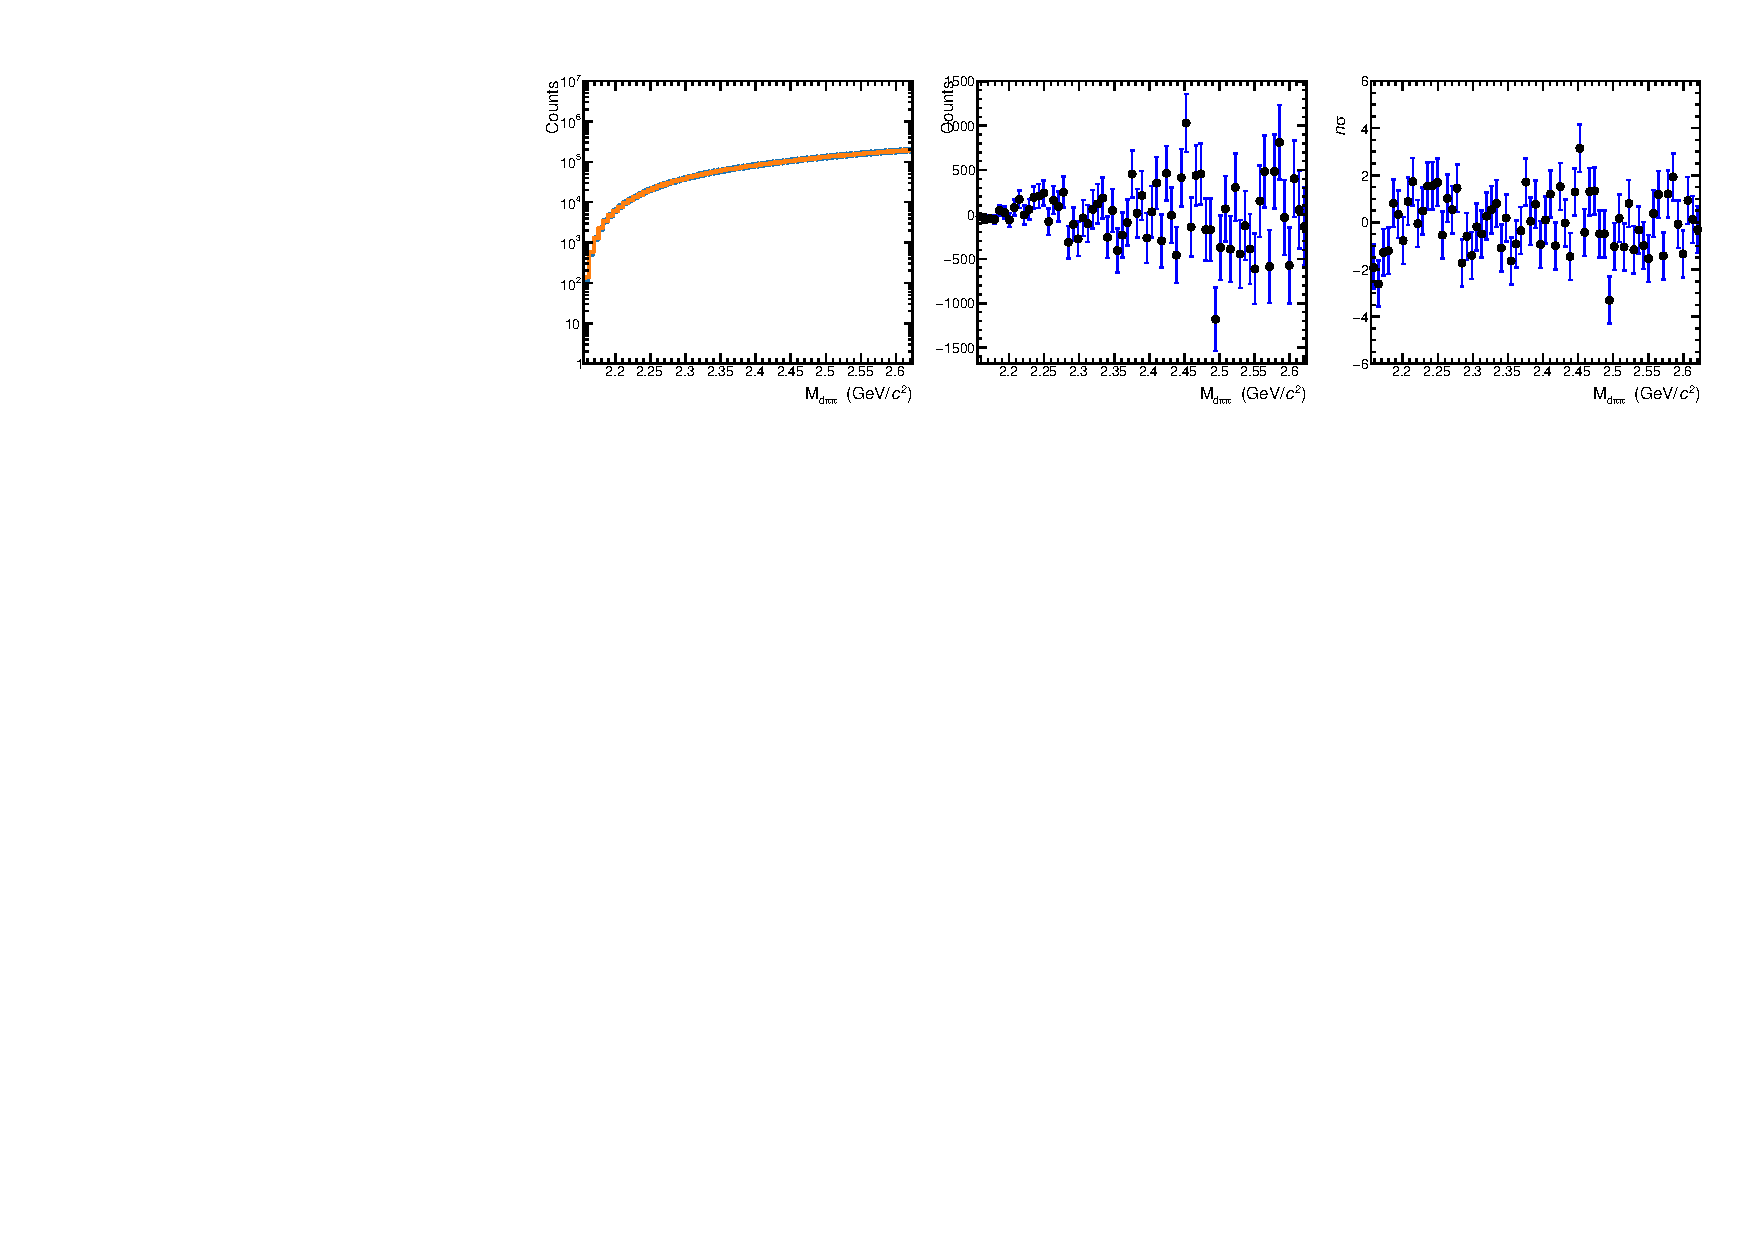
\includegraphics[width=\textwidth]{gfx/appendix/backsub/canvas5}
    \caption{Improved PEM model compared with \minv, in the $0.5 < \pt \leq 1.0$ \gevc interval. In the lower pad the data/model ratio is reported.}
    \label{fig:bs5}
\end{figure}



